\documentclass[11pt]{article}
 
\def\shownotes{1}
\def\blinded{0}


\usepackage[top=3cm, bottom=3cm, left=2cm, right=2cm]{geometry}      % [top=2cm, bottom=2cm, left=2cm, right=2cm]
\geometry{letterpaper}                   % ... or a4paper or a5paper or ...
%\geometry{landscape}                % Activate for for rotated page geometry
%\usepackage[parfill]{parskip}
\usepackage{graphicx}
\usepackage{amssymb, amsmath, amsfonts}
\usepackage{amsthm}
\usepackage{enumerate}
\usepackage{hyperref}
\usepackage{xspace}
\usepackage{graphicx}
\usepackage{latexsym}
\usepackage{color}
\usepackage{framed}
\usepackage{algpseudocode}

\mathchardef\mhyphen="2D

\newcommand{\supp}{\operatorname{supp}}

\newcommand{\secref}[1]{\mbox{Section~\ref{#1}}}
\newcommand{\subsecref}[1]{\mbox{Subsection~\ref{#1}}}
\newcommand{\apref}[1]{\mbox{Appendix~\ref{#1}}}
\newcommand{\thref}[1]{\mbox{Theorem~\ref{#1}}}
\newcommand{\exref}[1]{\mbox{Example~\ref{#1}}}
\newcommand{\defref}[1]{\mbox{Definition~\ref{#1}}}
\newcommand{\corref}[1]{\mbox{Corollary~\ref{#1}}}
\newcommand{\lemref}[1]{\mbox{Lemma~\ref{#1}}}
\newcommand{\assref}[1]{\mbox{Assumption~\ref{#1}}}
\newcommand{\probref}[1]{\mbox{Problem~\ref{#1}}}
\newcommand{\clref}[1]{\mbox{Claim~\ref{#1}}}
\newcommand{\propref}[1]{\mbox{Proposition~\ref{#1}}}
\newcommand{\remref}[1]{\mbox{Remark~\ref{#1}}}
\newcommand{\consref}[1]{\mbox{Construction~\ref{#1}}}
\newcommand{\figref}[1]{\mbox{Figure~\ref{#1}}}
\DeclareMathOperator*{\expe}{\mathbb{E}}
\DeclareMathOperator*{\var}{\text{Var}}
\DeclareMathOperator*{\argmax}{arg\,max}
  

\newcommand{\class}[1]{{\ensuremath{\mathsf{#1}}}}
\newcommand{\key}{\ensuremath{\class{key}}\xspace}
\newcommand{\Key}{\ensuremath{\class{Key}}\xspace}

\newcommand{\gen}{\ensuremath{\class{Gen}}\xspace}
\newcommand{\rep}{\ensuremath{\class{Rep}}\xspace}
\newcommand{\sketch}{\ensuremath{\class{SS}}\xspace}
\newcommand{\rec}{\ensuremath{\class{Rec}}\xspace}
\newcommand{\enc}{\ensuremath{\class{Enc}}\xspace}
\newcommand{\dec}{\ensuremath{\class{Dec}}\xspace}
\newcommand{\prg}{\ensuremath{\class{prg}}\xspace}
\newcommand{\crust}{\ensuremath{\class{Crust}}\xspace}
\newcommand{\inter}{\ensuremath{\class{Inter}}\xspace}
\newcommand{\zo}{\ensuremath{\{0, 1\}}}
\newcommand{\vect}[1]{\ensuremath{\mathbf{#1}}}
\newcommand{\zq}{\ensuremath{\mathbb{Z}_q}}
\newcommand{\Fq}{\ensuremath{\mathbb{F}_q}}
\newcommand{\sample}{\ensuremath{\class{Sample}}\xspace}
\newcommand{\neigh}{\ensuremath{\class{Neigh}}\xspace}
\newcommand{\dis}{\ensuremath{\mathsf{dis}}}
\newcommand{\decode}{\ensuremath{\mathsf{Decode}}}
\newcommand{\guess}{\mathsf{guess}}
\newcommand{\eqdef}{\stackrel{\rm def}{=}}


\newcommand{\A}{\mathcal{A}}


\newcommand{\metric}{\ensuremath{\mathtt{Metric}}\xspace}
\newcommand{\hill}{\ensuremath{\mathtt{HILL}}\xspace}
\newcommand{\hillrlx}{\ensuremath{\mathtt{HILL\mhyphen rlx}}\xspace}
\newcommand{\yao}{\ensuremath{\mathtt{Yao}}\xspace}
\newcommand{\unp}{\ensuremath{\mathtt{unp}}\xspace}
\newcommand{\unprlx}{\ensuremath{\mathtt{unp\mhyphen rlx}}\xspace}
\newcommand{\metricstar}{\ensuremath{\mathtt{Metric}^*}\xspace}
\newcommand{\metricd}{\ensuremath{\mathtt{Metric}^*\mathtt{-d}}\xspace}
\newcommand{\hillstar}{\ensuremath{\mathtt{HILL}^*}\xspace}
\newcommand{\hillprime}{\ensuremath{\mathtt{HILL'}}\xspace}
\newcommand{\metricprime}{\ensuremath{\mathtt{Metric'}}\xspace}
\newcommand{\metricprimestar}{\ensuremath{\mathtt{Metric'}^*}\xspace}
\newcommand{\hillprimestar}{\ensuremath{\mathtt{HILL'}^*}\xspace}
\newcommand{\poly}{\ensuremath{\mathtt{poly}}\xspace}
\newcommand{\rank}{\ensuremath{\mathtt{rank}}\xspace}
\newcommand{\ngl}{\ensuremath{\mathtt{ngl}}\xspace}
\newcommand{\Hoo}{\mathrm{H}_\infty}
\newcommand{\Hav}{\tilde{\mathrm{H}}_\infty}
\newcommand{\Hfuzz}{\mathrm{H}^{\mathtt{fuzz}}_{t,\infty}}
\newcommand{\Hfav}{\tilde{\mathrm{H}}^{\mathtt{fuzz}}_{t,\infty}}
\newcommand{\Hcorr}{\mathrm{H}^{\mathtt{corr}}}
\newcommand{\Huse}{\mathrm{H}_{\mathtt{usable}}}
\newcommand{\Dom}{\mathsl{Dom}}
\newcommand{\Range}{\mathsl{Rng}}
\newcommand{\Keys}{\mathsl{Keys}}
\def\col{\mathrm{Col}}

\newcommand{\ddetbin}{\ensuremath{\mathcal{D}^{det,\{0,1\}}}}
\newcommand{\drandbin}{\ensuremath{\mathcal{D}^{rand,\{0,1\}}}}
\newcommand{\ddetrange}{\ensuremath{\mathcal{D}^{det,[0,1]}}}
\newcommand{\drandrange}{\ensuremath{\mathcal{D}^{rand,[0,1]}}}

\newcommand{\expinfo}{\ensuremath{\mathcal{E}}}
\newcommand{\ext}{\ensuremath{\mathtt{ext}}}
\newcommand{\cext}{\ensuremath{\mathtt{cext}}}
\newcommand{\rext}{\ensuremath{\mathtt{rext}}}
\newcommand{\cons}{\ensuremath{\mathtt{cons}}}
\newcommand{\decons}{\ensuremath{\mathtt{decons}}}
\newcommand{\sd}{\ensuremath{\mathbf{SD}}}


\newcommand{\lwe}{\class{LWE}}
\newcommand{\LWE}{\class{LWE}}
\newcommand{\distLWE}{\ensuremath{\class{dist\mbox{-}LWE}}}

\newtheorem{theorem}{Theorem}[section]
\newtheorem{lemma}[theorem]{Lemma}
\newtheorem{proposition}[theorem]{Proposition}
\newtheorem{corollary}[theorem]{Corollary}
\newtheorem{definition}[theorem]{Definition}
\newtheorem{assumption}[theorem]{Assumption}
\newtheorem{claim}[theorem]{Claim}
\newtheorem{problem}[theorem]{Problem}
\newtheorem{construction}[theorem]{Construction}

\newcounter{ctr}
\newcounter{savectr}
\newcounter{ectr}

\newenvironment{newitemize}{%
\begin{list}{\mbox{}\hspace{5pt}$\bullet$\hfill}{\labelwidth=15pt%
\labelsep=5pt \leftmargin=20pt \topsep=3pt%
\setlength{\listparindent}{\saveparindent}%
\setlength{\parsep}{\saveparskip}%
\setlength{\itemsep}{3pt} }}{\end{list}}


\newenvironment{newenum}{%
\begin{list}{{\rm (\arabic{ctr})}\hfill}{\usecounter{ctr} \labelwidth=17pt%
\labelsep=5pt \leftmargin=22pt \topsep=3pt%
\setlength{\listparindent}{\saveparindent}%
\setlength{\parsep}{\saveparskip}%
\setlength{\itemsep}{2pt} }}{\end{list}}

\newenvironment{tiret}{%
\begin{list}{\hspace{2pt}\rule[0.5ex]{6pt}{1pt}\hfill}{\labelwidth=15pt%
\labelsep=3pt \leftmargin=22pt \topsep=3pt%
\setlength{\listparindent}{\saveparindent}%
\setlength{\parsep}{\saveparskip}%
\setlength{\itemsep}{2pt}}}{\end{list}}


\newenvironment{blocklist}{\begin{list}{}{\labelwidth=0pt%
\labelsep=0pt \leftmargin=0pt \topsep=10pt%
\setlength{\listparindent}{\saveparindent}%
\setlength{\parsep}{\saveparskip}%
\setlength{\itemsep}{20pt}}}{\end{list}}

\newenvironment{blocklistindented}{\begin{list}{}{\labelwidth=0pt%
\labelsep=30pt \leftmargin=30pt\topsep=5pt%
\setlength{\listparindent}{\saveparindent}%
\setlength{\parsep}{\saveparskip}%
\setlength{\itemsep}{10pt}}}{\end{list}}

\newenvironment{onelist}{%
\begin{list}{{\rm (\arabic{ctr})}\hfill}{\usecounter{ctr} \labelwidth=18pt%
\labelsep=7pt \leftmargin=25pt \topsep=2pt%
\setlength{\listparindent}{\saveparindent}%
\setlength{\parsep}{\saveparskip}%
\setlength{\itemsep}{2pt} }}{\end{list}}

\newenvironment{twolist}{%
\begin{list}{{\rm (\arabic{ctr}.\arabic{ectr})}%
\hfill}{\usecounter{ectr} \labelwidth=26pt%
\labelsep=7pt \leftmargin=33pt \topsep=2pt%
\setlength{\listparindent}{\saveparindent}%
\setlength{\parsep}{\saveparskip}%
\setlength{\itemsep}{2pt} }}{\end{list}}

\newenvironment{centerlist}{%
\begin{list}{\mbox{}}{\labelwidth=0pt%
\labelsep=0pt \leftmargin=0pt \topsep=10pt%
\setlength{\listparindent}{\saveparindent}%
\setlength{\parsep}{\saveparskip}%
\setlength{\itemsep}{10pt} }}{\end{list}}

\newenvironment{newcenter}[1]{\begin{centerlist}\centering%
\item #1}{\end{centerlist}}

\newenvironment{codecenter}[1]{\begin{small}\begin{centerlist}\centering%
\item #1}{\end{centerlist}\end{small}}

\ifnum\shownotes=1
\newcommand{\authnote}[2]{{\textcolor{red}{\textsf{#1 notes: }\textcolor{blue}{ #2}}\marginpar{\textcolor{red}{\textbf{!!!!!}}}}}
\else
\newcommand{\authnote}[2]{}
\fi

\ifnum\blinded=0
\newcommand{\blind}[1]{{#1}}
\else
\newcommand{\blind}[1]{}
\def\shownotes{0}
\fi


\newcommand{\bnote}[1]{{\authnote{Ben}{#1}}}
\newcommand{\lnote}[1]{{\authnote{Leo}{#1}}}
\newcommand{\anote}[1]{{\authnote{Adam}{#1}}}

\newcommand{\ve}{\vect{e}}
\newcommand{\vm}{\vect{m}}
\newcommand{\vy}{\vect{y}}
\newcommand{\vE}{\vect{E}}
\newcommand{\vS}{\vect{S}}
\newcommand{\vA}{\vect{A}}
\newcommand{\vc}{\vect{c}}
\newcommand{\vW}{\vect{W}}
\newcommand{\vQ}{\vect{Q}}
\newcommand{\vR}{\vect{R}}
\newcommand{\vU}{\vect{U}}
\newcommand{\vT}{\vect{T}}
\newcommand{\vX}{\vect{X}}
\newcommand{\vB}{\vect{B}}
\newcommand{\vz}{\vect{z}}
\newcommand{\vd}{\vect{d}}
\newcommand{\vs}{\vect{s}}
\newcommand{\vx}{\vect{x}}
\newcommand{\va}{\vect{a}}
\newcommand{\vb}{\vect{b}}
\newcommand{\vgamma}{\mathbf{\Gamma}}
\newcommand{\vt}{\vect{t}}
\newcommand{\vu}{\vect{u}}
\newcommand{\vF}{\vect{F}}
\newcommand{\recout}{x}
\newcommand{\ignore}[1]{}
\newcommand{\M}{\mathcal{M}}
\newcommand{\Vol}{\mathsf{Vol}}

\newcommand{\Succ}{\mathsf{Succ}}
\newcommand{\Adv}{\mathbf{Adv}}
 \newcommand{\Exp}{\mathbf{Exp}}

\title{When are Fuzzy Extractors Possible?}
\blind{
\author{
Benjamin Fuller\footnote{Email: {\tt bfuller@cs.bu.edu}.  Boston
  University and MIT Lincoln Laboratory.}  \and Leonid
Reyzin\footnote{Email: {\tt reyzin@cs.bu.edu}.  Boston University.}
\and Adam Smith\footnote{Email: {\tt asmith@cse.psu.edu}.
  Pennsylvania State University. This work performed while visiting Boston
  University's Hariri Institute for Computing.}}
}
\begin{document}
\maketitle

\begin{abstract}
Fuzzy extractors (Dodis et al., Eurocrypt 2004) convert repeated noisy readings of a high-entropy secret into the same uniformly distributed key. A minimum condition for the security of the key is the hardness of guessing a value that is similar to the secret, because the fuzzy extractor converts such a guess to the key.
We define \emph{fuzzy min-entropy} to quantify this property of a noisy source of secrets.  Fuzzy min-entropy measures the success of the adversary when provided with \emph{only} the functionality of the fuzzy extractor and thus the \emph{ideal} security possible from a noisy distribution.  

High fuzzy min-entropy is necessary for the existence of a fuzzy extractor; moreover, there is evidence that it may be sufficient when only computational security is required. Nevertheless, information-theoretic fuzzy extractors are not known for many practically relevant sources of high fuzzy min-entropy. The challenge is to design information-theoretic fuzzy extractors whose security (almost) matches the fuzzy min-entropy of a distribution.
In this work, we ask whether this challenge is inherent.
 We provide two main technical results.
\begin{itemize}
\item \textbf{Sufficiency of fuzzy min-entropy:}  We construct a fuzzy extractor for each physical source with fuzzy min-entropy.  This result justifies fuzzy min-entropy as the right measure of the quality of a noisy distribution for key derivation.  Previous results considered the entropy and error tolerance of a separately and had not secured many sources with fuzzy min-entropy.  The constructed fuzzy extractor must \emph{precisely know} the distribution of the noisy source.
\item \textbf{Cost of distributional uncertainty:}  High entropy sources can never be fully observed and must be modeled.  An adversary may have a better model than the fuzzy extractor designer.  To compensate, fuzzy extractors are typically designed to work for families of physical sources. We show that this uncertainty is an impediment to security by building a family of high fuzzy min-entropy sources for which no fuzzy extractor can exist.  This result emphasizes the importance of high fidelity models of high entropy sources.
\end{itemize}
We provide similar but stronger results for secure sketches, whose goal is not to derive a consistent key, but to recover a consistent reading of the secret.  Our results are information-theoretic, but we discuss implications for the computational setting. 

\medskip
\textbf{Keywords:} Fuzzy extractors, secure sketches, information theory, biometric authentication, error-tolerance, key derivation, error-correcting codes.
\end{abstract}

\newpage
%\tableofcontents\newpage

\section{Introduction}
Sources of reproducible secret random bits are necessary for many cryptographic applications.  In many situations these bits are not explicitly stored for future use, but are obtained by repeating the same process  (such as reading a biometric or a physically unclonable function) that generated them the first time.
However, bits obtained this way present a problem: noise \cite{daugman2004,zviran1993comparison,brostoff2000passfaces,ellison2000protecting,mayrhofer2009shake,monrose2002password,pappu2002physical,gassend2002silicon,tuyls2006puf,suh2007physical,bennett1988privacy}.  That is, when a secret is read multiple times, readings are close~(according to some metric) but not identical.  To utilize such sources, it is often necessary to remove noise, in order to derive the same value in subsequent readings.

The same problem occurs in the interactive setting, in which the secret channel used for transmitting the bits between two users is noisy and/or leaky~\cite{wyner1975wire}. Bennett, Brassard, and Robert~\cite{bennett1988privacy} identify two fundamental tasks.  The first, called information reconciliation, removes the noise without leaking significant information. The second, known as privacy amplification, converts the high entropy secret to a uniform random value.  In this work, we consider the noninteractive version of these problems, in which these tasks are performed together with a single message.

The noninteractive setting is modeled by a primitive called a fuzzy extractor~\cite{DBLP:journals/siamcomp/DodisORS08}, which consists of two algorithms.  %Consider some distribution $W$.%The goal of a fuzzy extractor is to derive stable keys from a distribution $W$ whenever the two readings~(denoted $w$ and $w'$ respectively) are within distance $t$.   T
The  generate algorithm ($\gen$)  takes an initial reading $w$ and produces an output $\key$ along with a nonsecret helper value $p$.  The reproduce~($\rep$) algorithm takes the subsequent reading $w'$ along with the helper value $p$ to reproduce $\key$.   The correctness guarantee is that the key is reproduced precisely as long as the distance between $w$ and $w'$ is at most $t$. 

The security requirement for fuzzy extractors is that $\key$ is uniform even to a (computationally unbounded) adversary who has observed $p$.   This requirement is  harder to satisfy as the allowed error tolerance $t$ increases, because it becomes easier for the adversary to guess $\key$ by guessing a $w'$ within distance $t$ of $w$ and running $\rep(w',p)$.


\paragraph{Fuzzy Min-Entropy}
We introduce a new entropy notion that precisely measures how hard it is for the adversary to guess a value within distance $t$ of the original reading $w$, thus subverting the security of $\key$ by running $\rep$. Suppose $w$ is sampled from a distribution $W$.   To have the maximum chance that $w'$ is within distance $t$ of $w$, the adversary would want to maximize the total probability mass of $W$ within the ball $B_t(w')$ of radius $t$ around $w'$.
We  therefore define \emph{fuzzy min-entropy} $\Hfuzz(W) \eqdef -\log \max_{w'} \Pr[W\in B_t(w')]$.  Observe that this quantity can be bounded in terms of min-entropy: $\Hoo(W) \ge \Hfuzz(W) \ge \Hoo(W)-\log |B_t|$.

Fuzzy min-entropy measures the quality of a distribution when provided oracle access to the functionality of a fuzzy extractor.  It can be thought of as measuring the ideal security of a noisy source of entropy when used for key derivation.  This is similar to how security is measured for program obfuscation~\cite{barak2001possibility}, we discuss the connection to program obfuscation in \secref{sec:related settings}.  Superlogarithmic fuzzy min-entropy is \emph{necessary} for nontrivial key extraction~(\propref{prop:fuzz necessary} formalizes the above intuition).  

However, existing constructions do not measure their security in terms of fuzzy min-entropy; instead, their security is shown to be  $\Hoo(W)$ minus some loss that is at least $\log |B_t|$ due to error-tolerance. Since $\Hoo(W)-\log |B_t| \le \Hfuzz(W)$, it is natural to ask whether this loss is necessary. This question is particularly relevant when the gap between the two sides of the inequality is high.\footnote{For nearly uniform distributions, $\Hfuzz(W) \approx \Hoo(W)- \log |B_t|$.  In this setting, standard coding based constructions of fuzzy extractors (instantiated with optimum codes) yield keys of size approximately $\Hfuzz(W)$.}  As an example, iris scans appear to have significant $\Hfuzz(W)$ (because iris scans for different people appear to be well-spread in the metric space~\cite{daugman2006probing}) but negative $\Hoo(W) -\log |B_t|$ \cite[Section 5]{blanton2009biometric}. We therefore ask: \emph{is fuzzy min-entropy sufficient for fuzzy extraction?} There is evidence that it may be when the security requirement is computational rather than information-theoretic---see \secref{sec:related settings}. We provide an answer in two settings.

\paragraph{Sufficiency of $\Hfuzz(W)$ for a Precisely Known Distribution}
Ideally, a fuzzy extractor has \emph{precise knowledge} of the probability distribution function of $W$.  We call this  the \emph{precise knowledge} setting.  In this setting, we show that for every source $W$ with superlogarithmic $\Hfuzz(W)$, it is possible to construct a fuzzy extractor with a superlogarithmic length $\key$ (\corref{cor:extension to fuzz ext}). Our construction crucially utilizes the probability distribution function of $W$ and, in particular, is not polynomial time.  This result shows that $\Hfuzz(W)$ is a necessary and sufficient condition for building a fuzzy extractor of a distribution $W$.  

A number of previous works in the precise knowledge setting have provided efficient algorithms and
tight bounds for specific distributions---generally the uniform distribution or
i.i.d. sequences (for example, \cite{JW99,LT03,DBLP:conf/eccv/TuylsG04,hao2006combining,DBLP:journals/corr/abs-1112-5630,IgnatenkoW2012}). 
Our characterization unifies previous work, and justifies using $\Hfuzz(W)$ as the measure of the quality of a noisy distribution,  rather than cruder measures such as $\Hoo(W)-\log |B_t|$. 

\paragraph{The Challenge of Precisely Knowing a High Entropy Distribution}
Assuming \emph{precise knowledge} of a distribution $W$ may be unrealistic. Indeed, high-entropy distributions can never be fully observed directly and must therefore be modeled. It is imprudent to assume that the designer's model of a distribution is completely accurate---the adversary, with greater resources, would likely be able to build a better model. Therefore, fuzzy extractor designs cannot usually be tailored to one  particular source. Existing designs work for a family of sources (for example, all sources of min-entropy at least $m$ with at most $t$ errors). Thus, the design is fixed with a partially known distribution, and the adversary may therefore know more about the distribution than the designer of the fuzzy extractor.  We call this setting \emph{distributional uncertainty}.
We ask whether fuzzy min-entropy is sufficient in each of these settings.

\paragraph{The Cost of Distributional Uncertainty}
When the distribution is $W$ is uncertain, our results are negative.   In this setting, $W$ is only known to be in family of distributions $\mathcal{W}_Z$.
We construct a family $\mathcal{W}_Z$ where not even a 2-bit fuzzy extractor can be secure for most distributions in  $\mathcal{W}_Z$.  We emphasize that each distribution $W_z\in \mathcal{W}_Z$ has superlogarithmic fuzzy min-entropy---in fact, $\Hfuzz(W_z)=\Hoo(W_z)$, because all points in $W_z$ are distance at least $t$ apart. Our proof relies on high dimensionality of each $W_z$ and on perfect correctness of the $\rep$ procedure.
This result shows that uncertainty in the distribution $W$ is devastating to building a fuzzy extractor.  In particular, our positive results (\corref{cor:extension to fuzz ext}) show it is possible to build a fuzzy extractor for each $W_z$, but no construction can simultaneously secure the whole family.  Our result motivates further research into high fidelity descriptions of noisy physical sources.

\begin{table}[h]
\begin{center}
\begin{tabular}{c  l l }
 & Precise Knowledge & Distributional Uncertainty\\
\hline
Fuzzy Extractor & Yes~(\corref{cor:extension to fuzz ext}) & No~(\thref{thm:imposs fuzz ext})\\
\hline
Secure Sketch & Yes~(\corref{cor:extension to fuzz ext}) & No~(\thref{thm:imposs sketch})
\end{tabular}
\end{center}
\caption{Is fuzzy min-entropy sufficient to extract a superlogarithmic length key?  Results are information-theoretic.}
\label{tab:main results}
\end{table}


\paragraph{Stronger Results on Information Reconciliation (Secure Sketches)}
Traditionally, fuzzy extractors use a secure sketch to perform information reconciliation~(mapping $w'$ back to $w$), followed by randomness extractor~\cite{nisan1993randomness} to transform $w$ into a uniform key.  The security losses incurred in the first of these two steps dominate for typical sources and, indeed, this step is less well understood.\footnote{Randomness extractors have matching upper and lower bounds on the security loss: for every extra two bits of output key, they lose one bit of security} Formally, a secure sketch performs non-interactive information reconciliation via pair of algorithms: $\sketch$ takes $w$ and produces a nonsecret value $ss$, while $\rec$ takes a value $w'$ within distance $t$ of $w$ and uses $\sketch$ to output the original reading $w$.  

We show comparable, but stronger, results for secure sketches.  Namely, we show in \corref{cor:extension to fuzz ext} that secure sketches are possible if the distribution $W$ is precisely known. (In fact, we obtain our fuzzy extractors for the case of a known distribution from this result by applying a randomness extractor.) 

On the other hand, there is a family of sources, $\mathcal{W}_Z$, where each element has $\Hfuzz(W_z)=\Hoo(W_z) = \omega(\log n)$ for which no secure sketch correcting even a few errors is possible~(\thref{thm:imposs sketch}). The impossibility result applies even when $\rec$ is allowed to be incorrect with probability up to $1/4$ (as opposed to our fuzzy extractor impossibility result). 

\bnote{compare to current constructions?}
\subsection{Our Techniques}

\paragraph{Techniques for Positive Results for a Precisely Known Distribution} We now explain how to construct a secure sketch for a precisely known distribution $W$ with fuzzy min-entropy (we already explained how to construct a fuzzy extractor from it).  We begin with distributions in which all points in the support have the same probability (so-called ``flat'' distributions).   Consider some subsequent reading $w'$. To achieve correctness, the sketch algorithm must disambiguate which point $w\in W$ within distance $t$ of $w'$ was sketched. Disambiguating multiple points can be accomplished by universal hashing, as long as the size of hash output space is slightly greater than the number of possible points. Thus, our sketch is computed via a universal hash of $w$. To determine the length of that sketch, consider the heaviest (according to $W$) ball of radius $t$. Because the distribution is flat, it is also the ball with the most points of nonzero probability. Thus, the length of the sketch needs to be slightly greater than the logarithm of the number of non-zero probability point in that ball. Since $\Hfuzz(W)$ is determined by the weight of that ball, the number of points cannot be too high and there will be entropy left after the sketch is published.

For an arbitrary distribution, we cannot afford to disambiguate points in the ball with the greatest number of points, because there could be too many low-probability points in a single ball despite a high $\Hfuzz(W)$.  We solve this problem by splitting the arbitrary distribution into a number of nearly flat distributions we call ``levels.''  We then write down, as part of the sketch, the level of the original reading $w$ and apply the above construction considering only points in that level.  We call this construction \emph{leveled hashing}~(\consref{cons:leveling}).

\paragraph{Techniques for Negative Results for Distributional Uncertainty}
We construct a family of distributions $\mathcal{W}_Z$ and prove impossibility for a uniformly random $W_z \leftarrow \mathcal{W}_Z$.
We start by observing the following asymmetry: $\gen$  sees only the sample $w$ (obtained via $W_z\leftarrow \mathcal{W}_Z$ and $w\leftarrow W_z$), while
the adversary knows $W_z$.   To exploit the asymmetry, we construct $\mathcal{W}_Z$ so that conditioning on the knowledge of $W_z$~(the outcome $z$) reduces the distribution to a single affine line, but conditioning on $w$ leaves the rest of the distribution uniform on a large fraction of the entire space.

Then we show how the adversary can exploit the knowledge of the affine line to reduce the uncertainty about $w$ (in the secure sketch case) or $\key$ (in the fuzzy extractor case). 
In the secure sketch case, $ss$ can be used to find fixed points of $\rec(\cdot, ss)$ which, by the correctness requirement of the sketch, must be separated by minimum distance $t$. This means there aren't too many of them, so few can lie on an average line, permitting the adversary to guess one easily.

In the fuzzy extractor case, the nonsecret value $p$ partitions the metric space into regions that produce a consistent value under $\rep$ (preimages of each $\key$ under $\rep(\cdot, p)$).  For each of these regions, the adversary knows that possible $w$ lie $t$-far from the boundary of the region.  However, in the Hamming space, the vast majority of points lie near the boundary (this follows by combining the isoperimetric inequality~\cite{harper1966optimal} showing that the ball has the smallest boundary and Hoeffding's inequality~\cite{hoeffding1963probability} for bounding the volume that is $t$-away from this boundary).  This allows the adversary to rule out so many possible $w$ that, combined with the adversarial knowledge of the affine line, many regions become empty, leaving $\key$ far from uniform.

The result for fuzzy extractors is delicate.  It uses the fact that $p$ partitions the space into nonoverlapping regions, which is implied by perfect correctness.  Extending this result to imperfect correctness seems challenging and is an interesting open problem. Our result also uses the fact that there are few points far from the boundary of every region, which is implied by the geometry of  the high-dimensional Hamming space.  This fact seems crucial: in contrast, in low-dimensional Euclidean space, which does not have this property, a single fuzzy extractor can work for any distribution with sufficient $\Hfuzz$. (Such a construction would use quantization or tiling, similar to, for example, \cite{CK03,LT03,CZC04,LC06,BDHTV10,VTOSS10}.  Each sample from $W$ would map to the ``tile'' containing it, from which the output key would be extracted. A randomly chosen quantizer would have the property that few samples lie near the boundary, giving almost-perfect correctness; if perfect correctness is desired, we can give up on security for those rare samples and simply use a special value of $p$ to indicate that one of them was the input.)

\subsection{Related Settings}
\label{sec:related settings}
\paragraph{Other settings with close readings:  $\Hfuzz$ is sufficient}
The security definition of fuzzy extractors and secure sketches can be weakened to protect only against computationally bounded adversaries~\cite{fuller2013computational}.   In this computational setting, a single fuzzy extractor (or secure sketch) can simultaneously secure all possible distributions by using virtual grey-box obfuscation for all circuits~\cite{BitanskyCKP14}. The construction places into $p$ the obfuscated program for testing proximity to $w$ and outputting the appropriate value if the test passes.  This construction is secure when the adversary can rarely learn \key with oracle access to the program functionality.  The set of distributions with fuzzy min-entropy are exactly those where an adversary learns \key with oracle access to the functionality with negligible probability.\footnote{If this construction is used for a secure sketch, $W$ will remain unpredictable conditioned on $p$, but will not have pseudoentropy (see  \secref{sec:feas comp sec sketch} for details).  Extending our negative result to the computational setting would rule out the existence of semantically-secure multilinear maps.}

Furthermore, the functional definition of fuzzy extractors and secure sketches can be weakened to permit interaction between the party having $w$ and the party having $w'$. Such a weakening is useful for secure remote authentication~\cite{Boyen05secureremote}. When both interaction and computational assumptions are allowed, secure two-party computation can produce a key that will be secure whenever the distribution $W$ has fuzzy min-entropy.  The two-party computation protocol needs to be secure without assuming authenticated channels; it can be built under the assumptions that collision-resistant hash functions and enhanced trapdoor permutations exist~\cite{DBLP:journals/joc/BarakCLPR11}.

\paragraph{Correlated rather than close readings}
A different model for the problem of key derivation from noisy sources does not explicitly consider the distance between $w$ and $w'$, but rather views $w$ and $w'$ as samples of drawn from a correlated pair of random variables.   This model is considered in multiple works, including~\cite{wyner1975wire,DBLP:journals/tit/CsiszarK78,DBLP:journals/tit/AhlswedeC93,DBLP:journals/tit/Maurer93}; recent characterizations of when key derivation is possible in this model include \cite{DBLP:conf/asiacrypt/RennerW05} and \cite{DBLP:journals/corr/TyagiW14}.  We compare our positive results to these characterizations in \apref{sec:corr variables}.  To the best of our knowledge, prior results on correlated random variables are in the precise knowledge setting, we are unaware of works that consider implications of distributional uncertainty.

%The definition of $\Hfuzz$ can be extended to this model (by again thinking of the adversary as choosing the value $w'$ that is most likely to lead to a success).

\paragraph{Organization} The remainder of the paper is organized as follows.  In \secref{sec:preliminaries}, we cover preliminaries and fuzzy extractor definitions.  In \secref{sec:known distributions}, we construct a fuzzy extractor in the precise knowledge setting.  In Sections~\ref{sec:family of dist} and~\ref{sec:imposs fuzz ext} we construct families of distributions that no secure sketches and fuzzy extractors can secure, respectively~(the distributional uncertainty setting).


\section{Preliminaries}
\label{sec:preliminaries}
%For a random variables $X_i$ over some alphabet $\mathcal{Z}$ we denote by $X = X_1,..., X_\gamma$  the tuple $(X_1,\dots, X_\gamma)$. % For a set of indices $J$, $X_{J}$ is the restriction of $X$ to the indices in $J$.  The set $J^c$ is the complement of $J$. 
Usually, we use capitalized letters for random variables and corresponding lowercase letters for their samples.
 Unless otherwise noted logarithms are base $2$.
The {\em min-entropy} of $W$ is $\Hoo(W) = -\log(\max_w \Pr[W=w])$,
and the {\em average (conditional)} min-entropy of $W$ given $P$ is  $\Hav(W|P) = -\log(\expe_{p\in P} \max_{w} \Pr[W=w|P=p])$~\cite[Section 2.4]{DBLP:journals/siamcomp/DodisORS08}.   Let $H_0(W)$ be the logarithm of the size of the support of $W$,  that is $H_0(W) = \log |\{w | \Pr[W=w]>0\}|$.  We use an average case of remaining support size $\tilde{H}_0(W |P) = \log ( \expe_{p\in P} |\{w | \Pr[W=w |P=p]>0\}|)$.

The {\em statistical distance} between random variables $X$ and $Y$ with the same domain is $\sd(X,Y) = \frac12 \sum_x |\Pr[X=x] - \Pr[Y=x]|$.
%For a distinguisher $D$ we write the \emph{computational distance} between $X$ and $Y$ as $\delta^D(X,Y) = \left| \expe[D(X)]-\expe[D(Y)]\right |$ (we extend it to a class of distinguishers $\mathcal{D}$ by taking the maximum over all distinguishers $D\in\mathcal{D}$).  We denote by $\mathcal{D}_{s}$ the class of randomized circuits which output a single bit and have size at most $s$.
For a metric space $(\mathcal{M}, \dis)$, the \emph{(closed) ball of radius $t$ around $w$} is the set of all points within radius $t$, that is, $B_t(w) = \{w'| \dis(w, w')\leq t\}$.  If the size of a ball in a metric space does not depend on $w$, we denote by $|B_t|$ the size of a ball of radius $t$.  We consider the Hamming metric over vectors in $\mathcal{Z}^\gamma$, defined via $\dis(w,w') = \{i | w_i \neq w'_i\}$ where $\mathcal{Z}$ is some alphabet.  For this metric, $|B_t| = \sum_{i=0}^t {\gamma \choose i} (|\mathcal{Z}|-1)^i $.  $U_\kappa$ denotes the uniformly  distributed random variable on $\{0,1\}^\kappa$.  Throughout this work, we consider a sequence of metric spaces $\mathcal{M}_n$ parameterized by $n$, but we write $\mathcal{M}$ for notational convenience. A \emph{negligible} function $\ngl(n)$ is one that decreases faster than any positive inverse polynomial as $n\rightarrow \infty$.

\subsection{Fuzzy Extractors and Secure Sketches}\label{sec:fuzz extractor}

In this section, we define fuzzy extractors and secure sketches.  Definitions and lemmas are drawn from the work of Dodis et al.~\cite[Sections 2.5--4.1]{DBLP:journals/siamcomp/DodisORS08} with modifications.  First, we allow for error as discussed in \cite[Section 8]{DBLP:journals/siamcomp/DodisORS08}.  Second, in the \emph{distributional uncertainty} setting we consider a general family $\mathcal{W}_Z$ of distributions instead of families containing all distributions of a given min-entropy.
%\footnote{Our negative results rule out a family that is a subset of all distributions with given min-entropy and thus rules out all distributions of a given entropy.}  
%This is a generalization of the definition of Dodis et al. which require a fuzzy extractor to work for all distributions of a particular entropy.  
%We discuss known distribution algorithms in \secref{sec:known distributions def}.  
Let $\mathcal{M}$ be a metric space with distance function $\dis$.

\begin{definition}
\label{def:fuzzy extractor}
An $(\mathcal{M}, \mathcal{W}_Z, \kappa, t, \epsilon)$-\emph{fuzzy extractor} with error $\delta$ is a pair of randomized procedures, ``generate'' $(\gen)$ and ``reproduce'' $(\rep)$. \gen on input $w\in \mathcal{M}$ outputs an extracted string $\key \in\{0,1\}^\kappa$ and a helper string $p\in\{0,1\}^*$. \rep takes $w'\in\mathcal{M}$ and $p\in\{0,1\}^*$ as inputs.   $(\gen, \rep)$ have the following properties:
\begin{enumerate}
\item \emph{Correctness:} if $\dis(w, w')\leq t$ and $(\key, p)\leftarrow \gen(w)$, then $\Pr[\rep(w', p) = \key] \geq 1-\delta$ (note that correctness holds for any $w'$ with probability $1-\delta$ over the coins on $\gen$ and $\rep$, but $w'$ cannot be a function of $p$).
\item \emph{Security:} for any distribution $W_z\in\mathcal{W}_Z$, if $(\Key,P)\leftarrow\gen (W_z)$, then $\sd((\Key,P),(U_\kappa,P))\leq \epsilon$.
\end{enumerate}
\end{definition}

\noindent
Fuzzy extractors perform two tasks, information-reconciliation and privacy amplification.  The standard construction is \emph{sketch-and-extract:} the uniform key is extracted from $w$~(using a randomness extractor~\cite{nisan1993randomness}) and the error-tolerance is obtained by using a secure sketch~\cite[Lemma 4.1]{DBLP:journals/siamcomp/DodisORS08}.  Secure sketches produce a string $ss$ that minimally decreases the entropy of $w$, while mapping nearby $w'$ to $w$:
\begin{definition}
\label{def:secure sketch}
An $(\mathcal{M},\mathcal{W}_Z, \tilde{m}, t)$-\emph{secure sketch} with error $\delta$ is a pair of randomized procedures, ``sketch'' $(\sketch)$ and ``recover'' $(\rec)$.  \sketch on input $w\in\mathcal{M}$ returns a bit string $ss\in\{0,1\}^*$.  \rec takes an element $w'\in\mathcal{M}$ and $ss\in\{0,1\}^*$.  $(\sketch, \rec)$ have the following properties:
\begin{enumerate}
\item \emph{Correctness}: $ \forall w, w'\in\mathcal{M}$ if $\dis(w,w')\leq t$ then $\Pr[\rec(w',\sketch(w))=w]\geq 1-\delta$ (note that correctness holds for any $w'$ with probability $1-\delta$ over the coins of $\sketch$ and $\rec$, but $w'$ cannot be a function of $\sketch(w)$).
\item \emph{Security}: for any distribution $W_z\in\mathcal{W}_Z$, $\Hav(W_z|\sketch(W_z))\geq \tilde{m}$.
\end{enumerate}
\end{definition}


\noindent
In the above definitions, the errors are chosen before $ss$ (resp., $p$) is known in order for the correctness guarantee to hold: correctness holds for any $w'$ with probability $1-\delta$ over the coins of the algorithms, but $w'$ cannot be a function of the output of  $\sketch(w)$. 


\paragraph{The Case of a Precisely Known Distribution}
If in the above definitions we take $\mathcal{W}_Z$ to be a one-element set containing a single distribution $W$, then the fuzzy extractor/secure sketch is said to be constructed for a \emph{precisely known distribution}.  In this case, we need to require correctness only for $w$ that have nonzero probability\footnote{We can extend correctness to all of $\mathcal{M}$ by defining $\gen$/$\sketch$ to output the point $w$ as part of $p/ss$ on zero-probability inputs, which will ensure that $\rep$/$\rec$ can always be correct; this does not affect security.}.

Note that we have no requirement that the algorithms are compact or efficient, and so the distribution can be fully known to them. Finding a natural model of specifying distributions that allows for efficient~(yet generic) known distribution constructions of sketches and extractors is an interesting problem.  

\paragraph{From Secure Sketches to Fuzzy Extractors}
A fuzzy extractor can be produced from a \emph{secure sketch} and an \emph{average case randomness extractor}:

\begin{definition}
Let $\mathcal{M}$, $\chi$ be finite sets.
A function $\ext: \mathcal{M}\times \{0,1\}^d \rightarrow \{0,1\}^\kappa$ a \emph{$(\tilde{m}, \epsilon)$-average case extractor} if for all pairs
of random variables $X, Y$ over $\mathcal{M}, \chi$ such that
$\tilde{H}_\infty(X|Y) \ge \tilde{m}$, we have $\sd((\ext(X, U_d), U_d, Y), U_\kappa\times
U_d \times Y) \le \epsilon$.
\end{definition}

\begin{lemma}
\label{lem:fuzzy ext construction}
Assume $(\sketch, \rec)$ is an $(\mathcal{M}, \mathcal{W}_Z, \tilde{m}, t)$-secure sketch with error $\delta$, and let $\ext:\mathcal{M}\times \zo^d \rightarrow \zo^\kappa$ be a $(\tilde{m}, \epsilon)$-average case extractor.  Then the following $(\gen, \rep)$ is an $(\mathcal{M}, \mathcal{W}_Z, \kappa, t, \epsilon)$-fuzzy extractor with error $\delta$:
\begin{itemize}
\item $\gen(w):$ generate $x\leftarrow \zo^d$, set $p=(\sketch(w), x), r=\ext(w;x)$, and output $(r,p)$.
\item $\rep(w', (s, x)):$ recover $w=\rec(w',s)$ and output $r=\ext(w;x)$.
\end{itemize}
\end{lemma}

\subsection{Fuzzy Min-Entropy: suitability of a noisy distribution for key derivation}
\label{sec:minimal conditions}
The value $p$ allows everyone, including the adversary, to find the output of $\rep(\cdot, p)$ on any input $w'$. Ideally,  $p$ should not provide any useful information beyond this ability, and the outputs of $\rep$ on inputs that are too distant from $w$ should provide no useful information, either.  In this ideal scenario, the adversary is limited to trying to guess a $w'$ that is $t$-close to $w$. 
Letting $w'$ be the center of the maximum-weight ball in $W$ would be optimal for the adversary.
We therefore measure the quality of a source by (the negative logarithm of) this weight.  

\begin{definition}
\label{def:fuzzy min-ent}
The $t$-fuzzy min-entropy of a distribution $W$ in a metric space $(\mathcal{M}, \dis)$ is:
\[
\Hfuzz(W) = -\log \left(\max_{w'}  \sum_{w\in W | \dis(w, w')\le t} \Pr[W=w] \right)
\]
\end{definition}
\noindent
Fuzzy min-entropy is a necessary condition for security.  It measures the advantage provided to the adversary by allowing them to run the $\rep$ functionality.  Thus, the fuzzy min-entropy is the ideal security that any fuzzy extractor should be compared against.  We defer proofs of statements in this section to \apref{sec:proof fuzz necessary}.
\begin{proposition}
\label{prop:fuzz necessary}
Let $W$ be a distribution  over $(\mathcal{M}, \dis)$ with $\Hfuzz(W) =m$.  Let $(\gen, \rep)$ be a $(\mathcal{M}, \{W\}, \kappa, t, \epsilon)$-fuzzy extractor with error $\delta$.  Then 
\[
\epsilon\ge 2^{-m}-\delta -2^{-\kappa}.
\]
In particular, for security parameter $n$, if $m = \Theta(\log n), \delta = \ngl(n), \kappa = \omega(\log n)$, then $\epsilon  = 1/\poly(n)$.
\end{proposition}

%Even if we consider a two party protocol where Alice holds $w$ and Bob holds $w'$, 
%\lemref{lem:fuzz necessary} still applies.  
The proof of \propref{prop:fuzz necessary} is not specific to the fuzzy extractor setting, it also applies to computational and interactive definitions.  Fuzzy min-entropy represents an upper bound on the security from a noisy source.  In the \secref{sec:related settings} computational setting there is evidence it may be possible to (nearly) achieve this upper bound.  However, in the information-theoretic setting there are many distributions with fuzzy min-entropy with no known fuzzy extractor~(or corresponding impossibility result).  We know show some properties of fuzzy min-entropy.
\begin{lemma}
\label{lem:conditional fuzz rule}
$\Hfuzz(W|P=p) \ge \Hfuzz(W) + \log \Pr[P=p]$.
\end{lemma}

\paragraph{Conditional Fuzzy min-entropy}
In our proofs, we will use a conditional version of fuzzy min-entropy.
\begin{definition}
\label{def:cond fuzzy ent}
The $t$-conditional fuzzy min-entropy of a distribution $W |P$ in a metric space $(\mathcal{M}, \dis)$ is:
\[
\Hfav(W|P) = -\log \left( \expe_{p\in P} \max_{w'} \sum_{w\in W |P =p | \dis(w, w')\le t} \Pr[W=w|P=p]\right).
\]
\end{definition}

\noindent

\begin{lemma}
\label{lem:chain rule fuzz}
$\Hfav(W|P) \ge \Hfuzz(W) - H_0(P)$.
\end{lemma}


\section{Sufficiency of $\Hfuzz(W)$ in the Precise Knowledge Setting}
\label{sec:known distributions}
In this section, we show it is possible to build secure sketches~(and thus fuzzy extractors through \lemref{lem:fuzzy ext construction}) given precise knowledge of a distribution $W$ whenever $\Hfuzz(W)= \omega(\log n)$.
We first consider flat distributions and then turn to arbitrary distributions.

\subsection{Flat Distributions}
A distribution is flat if all points in its support have the same probability. Let $\supp(W)$ denote the support of $W$, i.e., the set of points with nonzero probability.
\begin{definition}
A distribution $W$ is \emph{flat} if for all $w_0, w_1 \in \supp(W)$,  $\Pr[W=w_0] = \Pr[W=w_1]$.  
\end{definition}

Denote the largest number of points in a ball of radius $t$ in the support of $W$ as \[\beta_{t} = \max_{w'\in\M} |\{w | w\in \supp(W) \wedge \dis(w ,w')\le t\}|.\]   For flat distributions, this quantity defines the fuzzy min-entropy,
\begin{align}
\Hfuzz(W) &= -\log \left(\max_{w' \in \mathcal{M}} \left| \{w | w\in \supp(W) \wedge \dis(w, w')\le t\} \right|\cdot \Pr[W=w]\right) \nonumber \\
&= -\log\left( \max_{w' \in \mathcal{M}} |\{w | w\in \supp(W) \wedge \dis(w, w')\le t\}| \cdot 2^{-\Hoo(W)}\right) \nonumber \\
&= \Hoo(W) -\log \beta_{t}.\label{eq:fuzz for flat}
\end{align}

\noindent We use universal hashes to construct secure sketches for flat distributions.  Skoric et al. constructed secure sketches from universal hashes to correct a polynomial number of error patterns~\cite{skoric2009efficient}.


\begin{definition}[\cite{DBLP:journals/jcss/CarterW79}]
Let $F : \mathcal{K} \times \mathcal{M} \to R$ be a function.  We say that $F$ is \emph{universal} if for all distinct $x_1, x_2 \in \mathcal{M}$:
\[
 \Pr_{K \leftarrow \mathcal{K}}[F(K, x_1) = F(K, x_2)] = \frac{1}{|R|} \;.
\]
\end{definition}

\begin{construction}
\label{cons:universal hash}
Let $F :\mathcal{K}\times \mathcal{M}\rightarrow R$ be a universal hash function.  Let $W$ be a distribution.  Define $\sketch_W, \rec_W$ as:

\begin{center}
\begin{tabular}{c|c}
\begin{minipage}{2.5in}
\textbf{$\sketch_W$}
\begin{enumerate}
\item \underline{Input}: $w$.
\item Sample $K\leftarrow \mathcal{K}$.
\item Set $ss = F(K, w), K$.
\end{enumerate}
\vspace{.3in}
\end{minipage} &
\begin{minipage}{3.5in}
\textbf{$\rec_W$}
\begin{enumerate}
\item \underline{Input}: $(w', ss =( y, K))$
\item Let $W^* = \{w \in \supp(W) | \dis(w, w')\le t\}$.
\item For $w^*\in W^*$, if $F(K, w^*) = y$, \\ output $w^*$.
\item Output $\perp$.
\end{enumerate}
\end{minipage}
\end{tabular}
\end{center}
\end{construction}

\begin{lemma}
\label{lem:flat hashing} (Proof in \apref{sec:proof of flat hashing})
Let $W$ be a flat distribution with $\Hoo(W)\ge m$.  Then
\consref{cons:universal hash} is a $(\mathcal{M}, \{W\}, m - \log |R|, t)$-known distribution secure sketch with error $\delta \le \frac{\beta_{t}-1}{|R|}$. 
\end{lemma}
\begin{corollary}
Let $n = \log |\mathcal{M}|$.  If $|R| \ge |\beta_{t}|\cdot n^{\omega(1)}$ then \consref{cons:universal hash} is correct with overwhelming probability.  That is, setting $\log |R| = \log \beta_{t} + \omega(\log n)$ suffices.
\end{corollary}

\noindent
\consref{cons:universal hash} writes down enough information to disambiguate any ball of points.  The remaining entropy for this construction is $\Hav(W |\sketch(W)) = \Hoo(W) - \log \beta_{t} -\log 1/\delta$. For a flat distribution this is within a superlogarithmic factor of optimal~(see Equation~\eqref{eq:fuzz for flat}). By choosing $\delta$ based on $\Hfuzz(W)$ we build $(\sketch, \rec)$ such that $\Hav(W | \sketch(W)) = \omega(\log n)$.

\subsection{Arbitrary Distributions}
The hashing approach used in the previous subsection does not work for arbitrary sources.  The reason is that some balls may have  many points but low total weight. For example, let $W$ be a distribution consisting of the following balls. Denote by $B^1_t$ a ball with $2^{\Hoo(W)}$ points with probability $\Pr[W\in B^1_t] =2^{-\Hoo(W)}$.  Let $B^2_t,..., B^{2^{-\Hoo(W)}}_t$ be balls with one point each with probability $\Pr[W\in B^i_t] = 2^{-\Hoo(W)}$.  Then the hashing algorithm needs to write down $\Hoo(W)$ bits to achieve correctness on $B^1_t$.  However, with probability $1-2^{-\Hoo(W)}$ the initial reading is outside of $B^1_t$, and the hash completely reveals the point.  

Dealing with non-flat distributions requires a new strategy. 
Many solutions for manipulating high entropy distributions leverage a solution for flat distributions and use the fact that high entropy distributions are convex combinations of flat distributions.  However, a distribution with high fuzzy min-entropy may be formed from component distributions with little or no fuzzy min-entropy.  It is unclear how to leverage the convex combination property in this setting.  

The main obstacle in the arbitrary setting is distinguishing between a setting where a ball has a few high probability points and a large number of low probability points.
To overcome this problem, we write the probability of $w\in W$ in the sketch output.  To ensure this information does not completely reveal $w$ we write down only the approximate probability of the outcome $w$. We then use a universal hash whose output length is proportional to the maximum number of points of the same approximate probability in any ball.  

\begin{construction}
\label{cons:leveling}
Let $\mathcal{M}$ be a metric space and let $n =\log |\mathcal{M}|$. Let $W$ be a distribution with $\Hoo(W)= m$.  Let $\ell\in\mathbb{Z}^+$ be a parameter.  Let $L_i = (2^{-(i+1)}, 2^{-i}]$ for $i=m,..., m+\ell-1$.  Let $F_i :\mathcal{K}_i\times \mathcal{M}\rightarrow R_i$ be a parameterized family of universal hash functions.  Define $\sketch_W, \rec_W$ as: 
\begin{center}
\begin{tabular}{c|c}
\begin{minipage}{3in}
\textbf{$\sketch_W$}
\begin{enumerate}
\item \underline{Input}: $w$.
\item If $\Pr[W=w] \le 2^{-(m+\ell)}$. Set $ss=1,w$.
\item Else
\begin{enumerate}
\item Find $i$ such that $\Pr[W=w]\in L_i$.
\item Sample $K\leftarrow \mathcal{K}_i$.
\item Set $ss =0,  i, F_i(K, w), K$.
\end{enumerate}
\end{enumerate}
\vspace{.4in}
\end{minipage} &
\begin{minipage}{3.5in}
\textbf{$\rec_W$}
\begin{enumerate}
\item \underline{Input}: $(w', ss)$
\item If $ss_0 = 1$, output $ss_{1,..., |y|}$.
\item Else
\begin{enumerate}
\item Parse $(i, y, K) = ss_{1,..., |y|}$.
\item $W^* = \{w | \dis(w, w')\le t \\\, \, \, \wedge \Pr[W=w]\in L_i\}$.
\item For $w^*\in W^*$, if $F_i(K, w^*) = z$, \\ output $w^*$.
\item Output $\perp$.
\end{enumerate}
\end{enumerate}
\end{minipage}
\end{tabular}
\end{center}
\end{construction}

\noindent
To set parameters, we restrict our notation of the maximum likelihood ball to points of a given probability.  Define $\beta_{t,i}$ as the maximum number of points in a ball in level $i$.  That is,
\[
\beta_{t,i} = \max_{w' \in \mathcal{M}} \left|\{w | \dis(w, w')\le t \wedge \Pr[W=w]\in L_i\}\right|.
\]

\begin{theorem}
\label{thm:layered hashing}
Let $W$ be a distribution over $\mathcal{M}$ where $n =\log \M$.  Let $\delta>0$ be an function of $n$.  Let $F_i: \mathcal{K}_i \times \mathcal{M}\rightarrow R_i$ be a parameterized family of universal hash functions where $|R_i| = (\beta_{t,i}-1) /\delta$.  When $\ell = n$ \consref{cons:leveling} is a $(\mathcal{M}, \{W\}, \tilde{m}, t)$-known distribution secure sketch with error $\delta$ for $\tilde{m} = \Hfuzz(W) - \log n - \log 1/\delta - 4$.

\end{theorem}
\noindent
We provide a proof in \apref{sec:proof of layered hashing}.  The main idea is that providing the level information makes the distribution look nearly flat~(the probability of points differs by at most a factor of two).  We can apply similar techniques to \lemref{lem:flat hashing} to show security for each nearly flat distribution. Then, we show that providing the level information does not hurt security too much.

\begin{corollary}
\label{cor:extension to fuzz ext}
Let $\mathcal{M}$ be a sequence of metric space parameterized by $n$ where $n = \log |\M|$.
For any distribution $W$ over $\mathcal{M}$ with $\Hfuzz(W)=\omega(\log n)$, there exists a $(\mathcal{M}, \{W\}, \tilde{m}, t)$-known distribution secure sketch with $\tilde{m} = \omega(\log n)$ and $\delta = \ngl(n)$.  (Extendible to a fuzzy extractor using~\lemref{lem:fuzzy ext construction}.)
\end{corollary}

\section{Impossibility of Secure Sketches for a Family with $\Hfuzz$}
\label{sec:family of dist}

In the previous section, we showed the sufficiency of $\Hfuzz(W)$ when the distribution was precisely known.  It may be infeasible to completely characterize a high entropy distribution $W$.  Traditionally, algorithms deal with this \emph{distributional uncertainty} by providing security for a family of distributions $\mathcal{W}_Z$.  

In this section, we show distributional uncertainty of $W$ comes at a real cost.  The security game of a fuzzy extractor can be thought of as a three stage process: 1) the challenger specifies $(\sketch, \rec)$, 2) the adversary sees $(\sketch, \rec)$ and specifies $W_z\in \mathcal{W}_Z$ 3) the adversary wins if $\Hav(W_z|\sketch(W_z))< \tilde{m}$.  

We prove impossibility in a game that is harder for the adversary to win: 1) the challenger specifies $(\sketch, \rec)$ 2) the adversary samples a random distribution from $W_z\leftarrow \mathcal{W}_Z$ 3) the adversary wins if $\Hav(W_z|\sketch(W_z)) < \tilde{m}$.\footnote{Our results rule out security for an average member of $\mathcal{W}$.  It may be possible to improve parameters by ruling out only a worst case $W$.  In \apref{sec:def equiv}, we show that providing security for a family $\mathcal{W}$ is equivalent to providing security for all distributions over that family.}  

Let $V$ be the process of uniformly sampling $W_z\leftarrow \mathcal{W}_Z$ and then sampling $w\leftarrow W_z$.  Let the random variable $Z$ the outcome of sampling $W_z\leftarrow \mathcal{W}_Z$.  The view of the challenger is $V$, while the view of the adversary is $\sketch(V)$ and $Z$. 
We now show a family of distributions $\mathcal{W}_Z$ that does not admit a secure sketch.  

\begin{theorem}
\label{thm:imposs sketch}
Let $n$ be a security parameter.  There exists a family of distributions $\mathcal{W}_Z$ such that for each element $W_z\in \mathcal{W}_Z$, $\Hfuzz(W_z)= \omega(\log n)$, and yet for any $(\mathcal{M}, \mathcal{W}_Z, \tilde{m}, t)$-secure sketch $(\sketch, \rec)$ with error $\delta <1/4$ and distance $t\ge 4$, $\tilde{m}<2$.  

Furthermore, this is true on average.  Let $V$ be process of sampling $W_z\leftarrow \mathcal{W}_Z$ and sampling $w\leftarrow W_z$.  Then
\[
\Hav(V|\sketch(V), Z)< 2.
\]
\end{theorem}

\begin{proof}
We prove the stronger average case statement.
We first describe a family $\mathcal{W}_Z$.  Let $\mathbb{F}$ be some field of size $q =\omega(\poly(n))$.  
Let $\mathcal{W}_Z$ be the set of all distributions of the form 
\[w =  \begin{pmatrix} \vec{1} \\a_2  \\ \vdots \\ a_{\gamma} \end{pmatrix} w_1 + \begin{pmatrix} 0  \\ 
b_2\\ \vdots \\ b_{\gamma} \end{pmatrix} 
\]
The family is defined by the parameters $a_2,.., a_\gamma$ and $b_2,..., b_\gamma$ (seen by the adversary) and the distribution is sampled by sampling $w_1$.  Each distribution $W_z$ is an affine line in space $\mathbb{F}^\gamma$. The algorithm $\sketch, \rec$ never see $Z$ only the outcome of $v\leftarrow V$.
Fix some $4\le t < \gamma$.
We show the following~(in \apref{sec:proof secure sketch imposs}):

\begin{itemize}
\item \propref{prop:each element good}: for all $W_z\in \mathcal{W}_Z$, $\Hfuzz(W_z) = \omega (\log n)$. 
\item \propref{prop:distribution uniform}: the distribution $V$ is uniform.
\item \lemref{lem:secure sketch entropy loss}: for any secure sketch on $V$, the support size of $V | \sketch(V)$ decreases significantly.  Here we show the minimum distance between points of $V|\sketch(V)$ is at least $t$.
\item \lemref{lem:side info determines sketch}:  $\tilde{H}_0(V | \sketch(V), Z) < 2$.
\end{itemize}
\end{proof}
\noindent
\textbf{Note:} There is a tradeoff between the size of $\mathbb{F}$ and the error tolerance required for the counter example.  By increasing $t$ it is possible to show a counter example for a smaller $\mathbb{F}$.\bnote{it would be nice to say what our counter example says about the binary space.}
\subsection{Implications for Computational Secure Sketches}
\label{sec:feas comp sec sketch}
Fuller et al. showed that computational secure sketches that provide pseudoentropy imply information-theoretic secure sketches with almost the same parameters~\cite[Corollary 3.8]{fuller2013computational}.  %This means that ruling out any information-theoretic secure sketches also rules out a computational secure sketch.  
The definition of Fuller et al. uses a weak version of pseudoentropy~\cite{DBLP:journals/siamcomp/HastadILL99} due to Gentry and Wichs~\cite{gentry2011separating}.

\begin{definition}
\label{def:relaxed hill}
Let $(W, S)$ be a pair of random variables.  $W$ has 
\emph{relaxed HILL entropy} at least $\tilde{m}$ conditioned on $S$,
denoted $H^{\hillrlx}_{\epsilon_{sec}, s_{sec}}(W|S)\geq \tilde{m}$ if there exists a joint distribution $(X, Y)$, such that $\tilde{H}_\infty(X|Y)\geq \tilde{m}$ and $\delta^{\mathcal{D}_{s_{sec}}} ((W, S),(X,Y))\leq \epsilon_{sec}$.
\end{definition}

A \emph{HILL secure sketch} is obtained by replacing the security condition in \defref{def:secure sketch} with HILL entropy~(adding parameters $\epsilon_{sec}, s_{sec}$ to the definition, representing the distinguishing circuit).  By the contrapositive of~\cite[Corollary 3.8]{fuller2013computational}, no sketch can retain HILL entropy for the same family of distributions:

\begin{corollary}
\label{cor:imposs comp sketch}
Let $n$ be a security parameter and let $\mathcal{M} = |\mathbb{F}|^\gamma$.  There exists a family of distributions $\mathcal{W}_Z$ over $\mathcal{M}$ such that for each element $W_z\in \mathcal{W}_Z$, $\Hfuzz(W_z)= \omega(\log n)$ and for any $(\mathcal{M}, \mathcal{W}_Z, \tilde{m}, t)$-HILL secure sketch $(\sketch, \rec)$ that is $(s_{sec}, \epsilon_{sec})$-hard and error $\delta$.  If 
$s_{sec}\ge t(|\rec| + \gamma \log |\mathbb{F}|)$, 
$t\ge 4$, and 
 $\epsilon_{sec} + t\delta < 1/16$,
 then $\tilde{m} <4$.
\end{corollary}


%\begin{corollary}
%\label{cor:rec yields sketch}
%Let $\mathcal{Z}$ be an alphabet. Let $(\sketch', \rec')$ be an $(\epsilon,s_{sec})$-HILL-entropy $(\mathcal{Z}^n, n\log |\mathcal{Z}|, \tilde{m}, t)$-secure sketch with error $\delta$ for the Hamming metric over $\mathcal{Z}^n$, with $\rec'$ of circuit size $s_{rec}$.
%If $s_{sec}\geq t(s_{rec} + n\log |\mathcal{Z}|)$, then there exists a   $(\mathcal{Z}^n, n\log |\mathcal{Z}|, \tilde{m}-2,t)$ (information-theoretic) secure sketch with error
%$4(\epsilon+t\delta)$. 
%\end{corollary}

\noindent
Secure sketches that provide computational unpredictability are implied by virtual-grey box obfuscation of proximity functions~\cite{BitanskyCKP14}.  Our impossibility result says nothing about this weaker form of a secure sketch.  Extraction from unpredictability entropy can be done using an extractor with a reconstruction property~\cite{barak-computational, DBLP:conf/eurocrypt/HsiaoLR07}; however, in the computational setting, the obfuscated function can simply hide a randomly generated key, and therefore extraction is not necessary to obtain a fuzzy extractor.

\section{Impossibility of Fuzzy Extractors for a Family with $\Hfuzz$}
\label{sec:imposs fuzz ext}
In the previous section, we showed a family of distributions that does not admit a secure sketch.  We provide an analogous result for fuzzy extractors.  

\begin{theorem}
\label{thm:imposs fuzz ext}
Let $n$ be a security parameter.  There exists a family of distributions $\mathcal{W}_Z$ over $\zo^n$ satisfying the following conditions. For each element $W_z\in \mathcal{W}_Z$, $\Hfuzz(W_z)= \omega(\log n)$. Let $\kappa \ge 2$ and $t = \omega(n^{1/2}\log n)$.  Any $(\mathcal{M}, \mathcal{W}_Z, \kappa, t, \epsilon)$-fuzzy extractor with error $\delta = 0$ has $\epsilon > 1/8 - \ngl(n)$.

Furthermore, this is true on average.  Let $V$ be process of uniformly sampling $W_z\leftarrow \mathcal{W}_Z$ and sampling $w\leftarrow W_z$.  Let $(\Key, P)\leftarrow \gen(V)$.  Then, 
\[
\sd ((\Key,P, Z), (U_\kappa, P, Z))>1/8-\ngl(n)\,.
\]

\end{theorem}

\begin{proof}[Proof Outline]
We prove the stronger average case statement.
Let $\nu = \omega(\log n)$ and $\nu = o(n^{1/2}/\log n)$.  Let $t=4\nu n^{1/2}+1$ and note that $n/\nu >t$.  

Our counterexample uses a slightly different family of distributions $\mathcal{W}_Z$ than the counterexample for secure sketches.  
We will work over a binary alphabet~(we used a large alphabet in our counterexample for secure sketches).  A  property of the binary Hamming space is that a large fraction of any set of bounded size is the near ``boundary'' of that set.  This will be crucial in our proof.  We will embed the larger alphabet in the secure sketch counterexample into the binary Hamming metric.
Let $x_1,..., x_\nu \in \zo^\nu$.  Let $\mathbb{F}$ denote the field of size $2^{\nu}$.  Let $a_2,..., a_{n/\nu}\in\mathbb{F}$ such that $a_i\neq 0$ and let $b_2,..., b_{n/\nu}\in\mathbb{F}$.  
Interpret $x_1,..., x_{\nu}$ as a element $x\in \mathbb{F}$ and let 
\[w =  \begin{pmatrix} \vec{1} \\a_2  \\ \vdots \\ a_{n/\nu} \end{pmatrix} x + \begin{pmatrix} 0  \\ 
b_2\\ \vdots \\ b_{n/\nu} \end{pmatrix} .
\]
The multiplication is in $\mathbb{F}$.  The family $\mathcal{W}_Z$ is parameterized by $z = a_2,..., a_{n/\nu}, b_2,..., b_{n/\nu}$.  
A particular distribution $W_z$ is then the uniform distribution over choices of $x$.
 Define $V$ as the process of uniformly choosing $W_z\leftarrow \mathcal{W}_Z$ and then sampling from $w\leftarrow W_z$.  The adversary sees $\sketch(V)$  and $Z$.  We then show the following~(proofs in \apref{sec:fuzz ext proof}):
\begin{itemize}
\item \propref{prop:dist fuzzy ent fuzz}: for all $W_z\in \mathcal{W}_Z$, $\Hfuzz(W_z) = \omega (\log n)$. 
\item \propref{prop:dist uniform fuzz}: the distribution $V$ is uniform.
\item \lemref{lem:fuzz can't get key}: In expectation across $Z$, a large subset of keys that are not possible.  In more detail,
\begin{itemize}
\item Half the keys have at most $2^{n- \kappa}$ pre images in the metric space~(this is at most half the metric space).  Denote this set as $\Key_{small}$.  
\item Consider some $\key \in \Key_{small}$.  %Our goal is to show there are few values of $v \in V|Z$ that could produce this key.  
Consider the set of $V_{\key } = \{w | \rep(w, p) = \key \}$.  All points in $V | \sketch(V)$ are distance $t$ from a boundary of $V_\key$~(the functionality of $\rep$ guarantees that for the true $w$ all nearby points map to the same $\key$).  We show that most of $V_\key$ is near a boundary.  A result of Frankel and F{\"u}redi says that the boundary of a region is minimized by a ball containing the same number of points~\cite{frankl1981short}.  Hoeffding's inequality says that most of a ball lies near its boundary~\cite{hoeffding1963probability}.  The number of $w$ that could produce $\key$ is small.
\item There are many possible values for $z_1, z_2$ for the side information $Z$~(and these possible values are equally likely).  Furthermore, the distributions $V|Z=z_1 $ and $V| Z=z_2$ have disjoint support outside of a single point $w$.
\item For most values of possible $Z$, the intersection between the viable pre images of $V|Z$ and $V_\key$ contains at most one point~(the received point $v$).  Checking if $V|Z \cap V_{\key}$ is nonempty is an effective distinguisher.
\end{itemize}
\end{itemize}

\end{proof}

\noindent
\textbf{Note:} As stated in \secref{sec:related settings}, using strong computational assumptions it is possible to avoid this result.  We note that the specific family $\mathcal{W}_Z$, Canetti et al.~\cite[Construction 5.3]{canetti2014key} construct computational fuzzy extractors  for this family of distributions when $\mathbb{F}$ is large enough under weaker assumptions.  (Their construction is stated with imperfect correctness.  A construction with perfect correctness is obtained by using a code that corrects $t$ bidirectional errors instead of a code that corrects $t$ unidirectional errors.)

\paragraph{Comparison with \thref{thm:imposs sketch}} The parameters in this result are weaker than those in \thref{thm:imposs sketch}.  This result requires: 1) higher error tolerance $t= \omega(n^{1/2}\log n)$ 2) the fuzzy extractor must have perfect correctness.  The secure sketch counter example needs $t=4$ and allows the $\rec$ to be wrong almost $1/4$ of the time.

\section*{Acknowledgements}
The authors are grateful to Gene Itkis and Yevgeniy Dodis for helpful discussions.
The work of Benjamin Fuller is sponsored in part by US NSF grants 1012910 and 1012798 and  the United States Air Force under Air Force Contract FA8721-05-C-0002. Opinions, interpretations, conclusions and recommendations are those of the authors and are not necessarily endorsed by the United States Government. 
Leonid Reyzin is supported in part by US NSF grants 0831281, 1012910, 1012798, and 1422965.  Adam Smith is supported in part by NSF awards 0747294 and 0941553.


\bibliographystyle{alpha}
\bibliography{crypto}

\appendix

\section{Key Derivation from Correlated Random Variables}
\label{sec:corr variables}

In this work, we consider two draws from some physical source whose distance was bounded according to some metric space.
Instead of considering $w, w'$ that have bounded distance, we can treat $W, W'$ as a pair of correlated random variables.  
  Renner and Wolf~\cite{DBLP:conf/asiacrypt/RennerW05} study this setting, firsting consider information-reconciliation and privacy amplification separately.  They show that $\Hoo(W)$ is a necessary and sufficient condition for privacy amplification.\footnote{The results of Renner and Wolf use smooth notions of entropy.  A random variable has smooth entropy if it is statistically close to a distribution with true entropy. We describe their results in the terminology of non smooth entropy.}  Second, they show that the length of $p$ must grow with the worst case number of possible outcomes for $W$ conditioned on $W'$.\footnote{This result also uses a smooth notion of entropy.  We describe the non smooth version for simplicity.}  That is, the length of the public value \[|p|\ge \max_{w'\in W} \log |\{w | \Pr[W=w | W'=w']>0\}|.\]

Furthermore, they show there exists a protocol with this length $p$ using optimal encoding functions.  Intuitively, the public information must describe which possible outcome for $W$ actually occurred. This result describes the maximal length of $p$ and does not argue how $p$ effects security.  It may be possible to construct a $p$ that reduces the entropy of $w$ by less than $\log |p|$.  In \secref{sec:known distributions}, we will construct schemes with variable length $p$, providing information-reconciliation for distributions where the bounds of Renner and Wolf provide no security guarantees.

Lastly, the work of Renner and Wolf shows characterize when key derivation is possible from correlated random variables~\cite[Theorem 3]{DBLP:conf/asiacrypt/RennerW05}.  Fuzzy min-entropy can be generalized to this setting.   Fuzzy extractors consider the worst case $w'$.  When considering correlated readings, it is natural to treat $W'$ as a random variable:\footnote{Fuzzy extractors are defined to require high probability of correctness for all pairs $w, w'$.  In the correlated setting, it may make sense to provide an average-case guarantee, where the probability of correctness is also over the draw of $w, w'$.  Renner and Wolf use a smoothed notion of entropy that removes the $\delta$ fraction of the probability mass of $W=w|W'=w'$ with the most points to improve parameters under such a definition.  In this work, we consider worst case correctness and use unsmoothed entropy.}

\begin{definition}
\label{def:cor fuzz min}
Let $(W, W')$ be a pair of correlated random variables.  The correlated fuzzy min-entropy of $W, W'$ is:
\[\Hcorr(W, W') = -\log \left( \max_{w'\in \supp(W')}\sum_{w\in W | \Pr[W=w|W'=w']>0} \Pr[W = w] \right).\]
\end{definition}
\noindent 
In \defref{def:fuzzy min-ent}, the sum is implicitly over $W=w|W'=w'$ since we assume any $w'$ within distance $t$ is possible.  
In \secref{sec:known distributions} we showed sufficiency  of $\Hfuzz(W)$ for key derivation from noisy sources (\defref{def:fuzzy min-ent}). 

\paragraph{Connection to the characterization of~\cite{DBLP:conf/asiacrypt/RennerW05}}
Renner and Wolf characterize when it is possible to derive keys from correlated random variables~\cite[Theorem 3]{DBLP:conf/asiacrypt/RennerW05}.  They consider all possible (randomized) transforms $T, T'$ of $W, W'$ into a new pair of variables $V,V'$.  They show that \[|\key| \le \sup_{(V, V')\leftarrow (T(W), T'(W))}\left(  \Hoo(V | T') - \log \max_{v'\in V'} |\{v| \Pr[V=v|T' \wedge V'=v']>0\}|\right).\]  Furthermore, they show that there is a transformation that achieves a key of nearly this length.  The result is nonconstructive as there is no guidance on how to find the transforms $T, T'$.  Since there is no known bound on the length of $T, T'$ it is not clear how to search the transform space even with unlimited time.
\consref{cons:leveling} can be used to derive keys from correlated random variables.  The main change is to define \[W^* = \{w | \Pr[W=w | W'=w'] >0 \wedge \Pr[W=w]\in L_i\}.\]  
Our result shows if one is satisfied with obtaining a strong key when possible (our protocol has losses of $2\log 1/\epsilon + \log n+\log 1/\delta$), then a protocol is possible (and explicitly constructible) in the original space. 





%\section{Leveraging convex combinations?}
%\label{sec:convex comb}
%\bnote{be careful uncommenting this, some notation may be out of date}
%In many situations solving a problem for min-entropy distributions can be reduced to solving the problem for flat distributions and then using the fact that any min-entropy distribution is a convex combination of flat distributions.  For example, consider the following hypothetical extension to \consref{cons:universal hash}.  Let $W$ be some distribution that is a finite convex combination of flat sources $W_1,..., W_\alpha$ where each $\forall i, \Hoo(W_i)\ge k$.\footnote{A distribution may be an  convex combination of an infinite number of distributions.  However, the problem arises even when considering a finite combination so we restrict ourselves to this simpler case.}  For convenience we assume that the coefficients on all $W_i$ are the same and distributions may be repeated. 
%
%We now describe a possible modification to the hashing construction.  Upon receiving an input $w$, sample a distribution $W_i$ from the set of distributions where $w$ has nonzero probability, write $i$ and perform the sketch as before for distribution $W_i$.  Intuitively, writing down a distribution $i$ should not do any harm as each of distributions $W_i$ has the same min-entropy as the starting distribution.  Unfortunately, this proposal may remove all entropy.  %Furthermore, each of these distributions is flat and thus, \consref{cons:universal hash} should apply.  However, this is not the case.
%
%%In the flat case, we used a hash whose length was proportional to the number of points in the largest ball.  The residual entropy in this case was within a superlogarithmic factor of $\Hfuzz(W)$.  However, in the setting where $W$ is a convex combination of flat sources this does not hold.
%
%Consider set of distributions $W_i$ where each $W_i$ has two components, first $W_i$ contains a distinguished point $w^*$ where $\Pr[W=w^*] = 2^{-k}$ and $w^*$ has no neighbors and $W_i$ contains a set $B_i$ of $2^{-k}-1$ points within distance $t$ each with probability $2^{-k}$.  This distribution is illustrated in \figref{fig:convex comb}.  
%
%\begin{figure}
%
%\centering
%    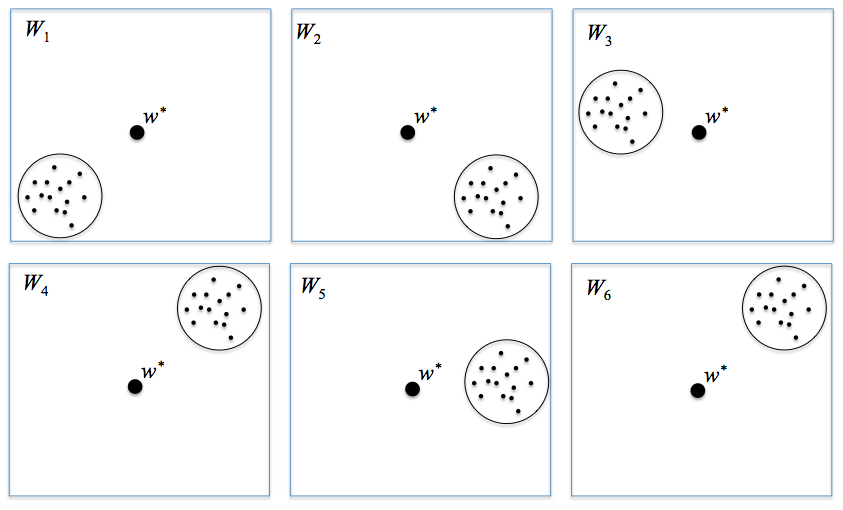
\includegraphics[width=.9\textwidth]{convexCombExample.png}
%    \caption{A convex combination of $W_1,..., W_\alpha$ has high min and fuzzy min-entropy, but sketching by using the component flat distributions removes all entropy.}
%\label{fig:convex comb}    
%\end{figure}
%
%
%The fuzzy min-entropy of $W_i$ is almost $0$ as the overwhelming majority of the probability space lies in $B_i$.  Now consider the distribution $W$ that is a convex combination of the $W_i$~(we assume that $B_i$ do not intersect).  Note that $\Hoo(W)=k$ and that $\Hfuzz(W)\approx \min\{\alpha, k\}$ where $\alpha$ is the number of distributions $W_1,..., W_\gamma$.  The value $\alpha$ may be quite large and $k$ may be the dominant factor.
%
%Consider an input point $w\in W$.  One of two cases occurs either $w=w^*$ or $w\in B_i$ for some $i$.  It should be clear in either case that the selected distribution $W_i$ is uniformly distributed from $\{1,..., \alpha\}$.  For any of the selected distributions, there is a ball with $\approx 2^{-k}$ points and thus the hash based construction must write down approximately $k$ points.  This means that $\Hav(W | \sketch(W))  = \Hav(W_i | \sketch(W_i)) \approx 0$.  This is despite the fact $\Hfuzz(W) \approx \min\{\gamma, k\}$.  Thus, the ability to sketch flat distributions does not easily admit a technique to sketch non-flat distributions.  
\bnote{I removed the discussion of convex combs for the submitted version}

\section{A Definitional Equivalence}
\label{sec:def equiv}
%We refer to $\mathcal{W}$ as the \emph{family}, the distribution $W$ as a \emph{source} and the particular outcome taken $w\in W$ as the \emph{sample}.   

As described in \secref{sec:family of dist}, our negative results rule out security for an average member of $\mathcal{W}$.  It may be possible to significantly improve parameters by only ruling out security for a single member $W$.  

Recall the security game of a fuzzy extractor: 1) the challenger specifies $(\sketch, \rec)$, 2) the adversary specifies a source $W\in \mathcal{W}$ 3) The challenger wins if $\Hav(W|\sketch(W))\ge \tilde{m}$.  Instead of just thinking of the uniform distribution over $\mathcal{W}$, consider an arbitrary distribution $V$ over elements of $\mathcal{W}$.  The minimax theorem says we can reverse which of these actions is announced first~\cite{neumann1928theorie} if $\mathcal{A}$ announces $V$ instead of a single element $W$.  That is, the following two player games have the same equilibrium:


\begin{center}
\begin{tabular}{c|c}
\begin{minipage}{3in}
\begin{tabbing}
123\=123\=123\=123\=123\=\kill
\textbf{Experiment} $\Exp^{\mathcal{W}}_1(\mathcal{A}, \mathcal{C}, \tilde{m})$: \\
$(\sketch, \rec)\leftarrow \mathcal{C}(\mathcal{W})$\\
$W \leftarrow \mathcal{A}(\mathcal{W}, \sketch, \rec)$\\
If $W\not\in \mathcal{W}$, $\mathcal{C}$ wins.\\
If $\Hav(W | \sketch(W))\ge \tilde{m}$, $\mathcal{C}$ wins.\\
Else $\mathcal{A}$ wins.
\end{tabbing} 
\vspace{.065in}
\end{minipage}  &
\begin{minipage}{3in}
\begin{tabbing}
123\=123\=123\=123\=123\=\kill
\textbf{Experiment} $\Exp^{\mathcal{W}}_2(\mathcal{A}, \mathcal{C}, \tilde{m})$: \\
$V \leftarrow \mathcal{A}(\mathcal{W})$\\
$(\sketch, \rec)\leftarrow \mathcal{C}(V, \mathcal{W})$\\
$W \leftarrow V$\\
If $W\not\in \mathcal{W}$, $\mathcal{C}$ wins.\\
If $\Hav(W | \sketch(W))\ge \tilde{m}$, $\mathcal{C}$ wins.\\
Else $\mathcal{A}$ wins.
\end{tabbing}
\end{minipage}
\end{tabular}
\end{center}

%The difference between these two games is which player announces their action first, in $\Exp^{\mathcal{W}}_1$, the challenger announces a pair of algorithms and the adversary specifies a source.  In $\Exp^{\mathcal{W}}_2$, the adversary specifies a distribution $V$ over sources, and the challenger then specifies their algorithm.  
This means that showing security for a family of distributions $\mathcal{W}$ is equivalent to showing security for all  distributions $V$ when the distribution is known to the algorithms $V$.  In our negative results, the adversary  uses the uniform distribution $V$ over $\mathcal{W}$.  However, it may be possible to improve parameters by using a different $V$. This would just rule out some member of $\mathcal{W}$ not an average member.  This is true for fuzzy extractors as well and is resilient to changes in parameters including imperfect correctness.


%Since the distribution used in our negative results was uniform it is stronger, ruling out security for an average $\mathcal{W}$.  However, constructing a nonuniform $V$ may improve these results.
%\begin{lemma}
%\label{lem:quant switch fuzz}
%Let $\mathcal{W}$ be a family of distributions.  If for all adversaries $\mathcal{A}$, there Let $(\sketch, \rec)$ be a $(\mathcal{M}, \mathcal{W}, \tilde{m}, t)$-secure sketch.  Let $V$ be a distribution over $\mathcal{W}$.  Then there exists $(\sketch', \rec')$ that is a $(\mathcal{M}, V, \tilde{m}, t)$-secure sketch on the mixed distribution $V$ when the adversary knows the sampled distribution $W$.\footnote{The other direction of this lemma is true as well.  If it is possible to construct a fuzzy extractor for an arbitrary distribution over a family then it is possible to construct a fuzzy extractor for every element of the family.}
%\end{lemma}


%\begin{corollary}
%\label{cor:no fuzz for dist}
%Let $\mathcal{W}$ be a family of distributions.  Let $V$ be an arbitrary distribution over elements of $\mathcal{W}$.  If there does not exist a $(\mathcal{M}, V, \tilde{m}, t)$-secure sketch on the mixed distribution $V$, then there is no $(\mathcal{M}, \mathcal{W}, \tilde{m}, t)$-secure sketch.
%\end{corollary}
%
%Both \lemref{lem:quant switch fuzz} and \corref{cor:no fuzz for dist} apply for fuzzy extractors as well as secure sketches.  Additionally they generalize to imperfect correctness.
\section{Fuzzy min-entropy}
\label{sec:proof fuzz necessary}
In this section, we provide proofs of the items in \secref{sec:minimal conditions}.  
\begin{proof}[Proof of \propref{prop:fuzz necessary}]
Let $W$ be a distribution where $\Hfuzz(W) = m$.  This means that there exists a point $w' \in \mathcal{M}$ such that $\Pr_{w\in W}[\dis (w, w')\leq t] = 2^{-m}$.  Consider the following distinguisher $D$:
\begin{itemize}
\item Input $\key, p$.
\item If $\rep(w', p) = \key$, output $1$.
\item Else output $0$.
\end{itemize}
Clearly, $\Pr[D(\Key, P) = 1]\geq 2^{-m} - \delta$, while $\Pr[D(U_\kappa, P)=1 ]= 1/2^{-\kappa}$.  Thus,
\[
\sd((\Key, P), (U_\kappa, P)) \ge \delta^D((\Key, P), (U_\kappa, P))\geq 2^{-m} -\delta -2^{-\kappa}.
\]
This completes the proof of \propref{prop:fuzz necessary}.
\end{proof}
\begin{proof}[Proof of \lemref{lem:conditional fuzz rule}]
\begin{align*}
\Hfuzz(W | P=p) &= -\log \left(\max_{w'}  \sum_{w\in (W |P=p) | \dis(w, w')\le t} \Pr[W=w | P=p] \right)\\
 &= -\log \left(\max_{w'}  \sum_{w\in (W |P=p) | \dis(w, w')\le t} \frac{\Pr[W=w \wedge P=p]}{\Pr[P=p]} \right)\\
% &\ge -\log \left(\max_{w'}  \sum_{w\in (W |P=p) | \dis(w, w')\le t} \frac{\Pr[W=w]}{\Pr[P=p]} \right)\\
 &\ge -\log \left(\max_{w'}  \sum_{w\in W| \dis(w, w')\le t} \frac{\Pr[W=w]}{\Pr[P=p]} \right)\\
 &= \Hfuzz(W) + \log \Pr[P=p].
\end{align*}
This completes the proof of \lemref{lem:conditional fuzz rule}.
\end{proof}


\begin{proof}[Proof of \lemref{lem:chain rule fuzz}]
\begin{align*}
\Hfav(W|P) &= -\log \left( \expe_{p\leftarrow P} \max_{w'} \sum_{w\in W |P =p | \dis(w, w')\le t} \Pr[W=w|P=p] \right)\\
&= -\log \left( \sum_{p} \max_{w'} \sum_{w\in W |P =p | \dis(w, w')\le t} \Pr[W=w|P=p]\Pr[P=p] \right)\\
&= -\log \left( \sum_{p} \max_{w'} \sum_{w\in W |P =p | \dis(w, w')\le t} \Pr[W=w \wedge P=p] \right)\\
&\ge -\log \left( \sum_{p} \max_{w'} \sum_{w\in W |P =p | \dis(w, w')\le t} \Pr[W=w] \right)\\
&\ge -\log \left( \sum_{p} \max_{w'} \sum_{w\in W | \dis(w, w')\le t} \Pr[W=w] \right)\\
&\ge -\log \left( 2^{H_0(P)} \left(\max_{w'} \sum_{w\in W | \dis(w, w')\le t} \Pr[W=w] \right)\right)\\
&\ge \Hfuzz(W) - H_0(P).
\end{align*}
This completes the proof of \lemref{lem:chain rule fuzz}.
\end{proof}



\section{Proof of \lemref{lem:flat hashing}}
\label{sec:proof of flat hashing}
\begin{proof}
We first argue security.  Fix some $W\in\mathcal{W}$. Since $\mathcal{K}$ and $W$ are independent $\Hav(W | \mathcal{K}) = \Hoo(W) = m$.  Then by \cite[Lemma 2.2b]{DBLP:journals/siamcomp/DodisORS08}, $\Hav(W | \mathcal{K}, F(\mathcal{K}, W)) \ge \Hoo(W) - \log |F(\mathcal{W}, W)| \ge m - \log |R|$.

We now argue correctness.  Fix some $w, w'$.  Let $W^*$ denote the set of elements in $W$ within distance $t$ of $w'$.  The size of $W^*$ is at most $\beta_{t}$.  Since $w, w'$ are independent of $\sketch$ this set is independent of the choice of $\mathcal{K}$.  The algorithm  $\rec$ will never output $\perp$ as the correct $w$ will match the hash.  The probability that another element $w^*$ collides is:
\begin{align*}
\Pr[\exists w^* \in W^* |w^* \neq w \wedge F(K, w^*) = F(K, w)] &\le \sum_{w^*\in W^* | w^*\neq w} \Pr[F(K, w^*) = F(K, w)] \\
 &= \sum_{w^*\in W^* | w^*\neq w} \frac{1}{|R|} \le \frac{\beta_{t}-1}{|R|}
\end{align*}
The inequality proceeds by union bound. The first equality proceeds by the universality of $F$ and the second inequality proceeds by noting the number of wrong neighbors is bounded by $\beta_{t}-1$.  This completes the proof.
\end{proof}

\section{Proof of \thref{thm:layered hashing}}
\label{sec:proof of layered hashing}
\begin{proof}
Throughout the proof we assume that $\ell = n$ is the number of levels.  The proof can be carried out for an arbitrary $\ell$ but it leads to a complicated theorem statement.

\paragraph{Correctness:}  Fix some $w, w'$.  If $\Pr[W=w]\le 2^{-(m+\ell)} = 2^{-(m+n)}$, then $w$ is simply transmitted to $\rec$ and correctness is clear.  When $\Pr[W=w]> 2^{-(m+n)}$ let $L_i^*$ be the level of $\Pr[W=w]$.

Let $W^*$ denote the set of elements of $W$ in $L_i$ within distance $t$ of $w'$.  The size of $W^*$ is at most $\beta_{t,i}$. The choice of $w, w'$ is independent of $\sketch$, so this set is independent of $\mathcal{K}_i$~(it does effect the value of $i$ but not the particular outcome from $\mathcal{K}_i$).  The probability that another element $w^*$ matches the hash is:
\begin{align*}
\Pr[\exists w^* \in W^* |w^* \neq w \wedge F(K, w^*) = F(K, w)] &\le \sum_{w^*\in W^* | w^*\neq w} \Pr[F(K, w^*) = F(K, w)] \\
 &= \sum_{w^*\in W^* | w^*\neq w} \frac{1}{|R_i|} \le \frac{\beta_{t,i}-1}{|R_i|} = \delta
\end{align*}
The first inequality is by union bound. The first equality follows from the universality of $F$.  The second inequality follows since the number of neighbors is bounded by $\beta_{t,i}$.  

\paragraph{Security:}
We now argue security of the construction.  First note that the total weight of points whose probability is less than $2^{-(n+m)}$ is at most $2^{-m}$~(there are at most $2^n$ points in the distribution).  Let $1_{\text{low}}$ be the indicator random variable for $\Pr[W=w]\le 2^{-(n+m)}$.  Then 
\begin{align}
\Hav(W | \sketch(W)) &= -\log \left(\Pr[1_{\text{low}}=1] * 1 + \Pr[1_{\text{low}} =0]   2^{-\Hav(W | \sketch(W) \wedge 1_{\text{low}} = 0)}\right)\nonumber\\
&\ge -\log\left( 2^{-m} + (1-2^{-m})2^{-\Hav(W | \sketch(W) \wedge 1_{\text{low}} = 0)}\label{eq:min-entropy}\right)
\end{align}
For the remainder of the proof, we seek a bound on $\Hav(W | \sketch(W) \wedge 1_{\text{low}} =0).$  Let $L_I$ be the random variable of the level information (in what follows, $L_I$ takes values between $m$ and $m+n$, where possible we omit this for notational clarity). 

\begin{align}
\Hav(W | \sketch(W) \wedge 1_{\text{low}} =0) &=-\log \left( \expe_{i} 2^{-\Hav(W | \sketch(W) \wedge 1_{\text{low}}=0 \wedge L_I =i }) \right)\nonumber\\
&=-\log \left( \expe_{i} 2^{-\Hav(W | \mathcal{K}_i \wedge F_i(K_i, W) \wedge 1_{\text{low}}=0 \wedge L_I=i)}\right)\nonumber\\
&=-\log \left( \expe_{i} 2^{-\Hav(W |  F_i(K_i, W) \wedge 1_{\text{low}}=0 \wedge L_I=i)}\right)\nonumber\\
&\ge-\log \left( \expe_{i} 2^{-(\Hav(W |  1_{\text{low}}=0 \wedge L_I=i)-\log (\beta_{t, i}-1) +\log \delta)}\right)\nonumber\\
&\ge-\log \left(\frac{1}{\delta} \expe_{i} 2^{-(\Hav(W |  1_{\text{low}}=0 \wedge L_I=i)-\log (\beta_{t, i}-1))}\right)\nonumber\\
&\ge-\log \left(\expe_{i} 2^{-(\Hav(W |  1_{\text{low}}=0 \wedge L_I=i)-\log (\beta_{t, i}-1))}\right) - \log \frac{1}{\delta}\nonumber\\
&\ge-\log \left(\expe_{i} 2^{-(\Hav(W |  1_{\text{low}}=0 \wedge L_I=i)-\log (\beta_{t, i}))}\right) - \log \frac{1}{\delta}\label{eq:fuzzy ball size}
\end{align}

\noindent
The third line follows because the only dependence between $\mathcal{K}_i$ and $W$ is in $i$.  The fourth line follows by \cite[Lemma 2.2]{DBLP:journals/siamcomp/DodisORS08}.  We now show that the fuzzy min-entropy conditioned on the level information is proportional to $\beta_{t, i}$.  For convenience denote by $J \overset{def}= (L_I \wedge 1_{\text{low}}=0)$.  That is, $\Pr[J=i] \overset{def}= \Pr[1_{\text{low}}=0 \wedge L_I=i$]. 
\begin{claim}
\label{cl:fuzz proportional beta}
$\Hoo(W |   J=i ) -\log \beta_{t, i} \ge \Hfuzz(W | J=i)-1.$
\end{claim}
\begin{proof}
\begin{align*}
\Hfuzz(W|J=i) &= -\log \left(\max_{w' \in \mathcal{M}} \left( \sum_{w\in W | \Pr[W=w]\in L_i \wedge \dis(w, w')\le t} \Pr[W=w | J=i]\right) \right)\\
&\le -\log \left(\max_{w' \in \mathcal{M}} \left( \sum_{w\in W | \Pr[W=w]\in L_i \wedge \dis(w, w')\le t}\left( \min_{w^*\in W=w| J=i}\Pr[W=w^* | J=i]\right) \right)\right)\\
&\le -\log \left(\max_{w' \in \mathcal{M}} \left( \sum_{w\in W | \Pr[W=w]\in L_i \wedge \dis(w, w')\le t} \left(\max_{w^*\in W=w| J=i}\Pr[W=w^* | J=i]\right) \right)\right)+1\\
&= -\log \left(\max_{w' \in \mathcal{M}} \left( \sum_{w\in W | \Pr[W=w]\in L_i \wedge \dis(w, w')\le t} 2^{-\Hoo(W|J=i)}\right) \right)+1\\
&= \Hoo(W|J=i)- \log\left(\max_{w' \in \mathcal{M}} \left( \sum_{w\in W | \Pr[W=w]\in L_i \wedge \dis(w, w')\le t} 1\right) \right)+1\\
&=\Hoo(W|J=i)-  \log \left(\max_{w' \in \mathcal{M}} \left|\{w | \dis(w, w')\le t \wedge \Pr[W=w]\in L_i\}\right|\right)+1\\
&=\Hoo(W|J=i)+1-\log \beta_{t, i}.
\end{align*}
Where the third line follows by \lemref{lem:nearly flat after conditioning}, which follows the proof of \thref{thm:layered hashing}.  This completes the proof of \clref{cl:fuzz proportional beta}.
\end{proof}

\noindent 
We now return to the proof of \thref{thm:layered hashing}. Together Equation \ref{eq:fuzzy ball size} and \clref{cl:fuzz proportional beta} yield:
\begin{align*}
\Hav(W | \sketch(W) \wedge 1_{\text{low}} =0) &=-\log \left( \expe_{i} 2^{-\Hfuzz(W | I=i \wedge 1_{\text{low}}=0)-1}\right) -\log \frac{1}{\delta} \\
&=-\log \left( \expe_{i} 2^{-\Hfuzz(W | I=i \wedge 1_{\text{low}} =0)}\right) -1- \log \frac{1}{\delta} \\
&=\Hfav(W | I \wedge 1_{\text{low}}=0)-1- \log \frac{1}{\delta} \\
&\ge\Hfuzz(W | 1_{\text{low}}=0)-1-\log n -\log \frac{1}{\delta}\\
&\ge\Hfuzz(W)-1-\log n -\log \frac{1}{\delta} - \log (1-2^{-m})
\end{align*}
Where the second-to-last line follows by \lemref{lem:chain rule fuzz}.  The last line follows by \lemref{lem:conditional fuzz rule} and by noting that $\Pr[1_{\text{low}}=0] \ge 1/(1-2^{-m})$.
Returning to equation \ref{eq:min-entropy} one has:
\begin{align*}
\Hav(W | \sketch(W)) &\ge -\log\left( 2^{-m} + (1-2^{-m}) 2^{-\Hav(W | \sketch(W) \wedge 1_{\text{low}} = 0)}\label{eq:min-entropy}\right)\\
&\ge -\log \left(2^{-m}+2^{-(\Hfuzz(W) -1 - \log n  -\log 1/\delta-2\log (1-2^{-m}) )}\right)\\
&\ge -\log \min\{2^{-m}, 2^{-(\Hfuzz(W) -1 - \log n  -\log 1/\delta-2\log (1-2^{-m}) )}\}-1\\
&\ge \Hfuzz(W) - 2- \log n - \log 1/\delta  -2\log (1-2^{-m}) \\
&\ge \Hfuzz(W) - 4- \log n - \log 1/\delta
\end{align*}
Where the fourth line follows from the third because $\Hfuzz(W)\le \Hoo(W) = m$. The last line follows from the fourth because if $m\ge 1$, then $\log (1-2^{-m}) \le 1$ and if $m<1$ the entire bound is vacuous as $\Hfuzz(W) < 1$.
\end{proof}

\begin{lemma}
\label{lem:nearly flat after conditioning}
Let $W$ be a distribution and let $S\subset W$ such that for all $w_1, w_2 \in S$, $\Pr[W=w_1]\ge \Pr[W=w_2]$.  Let $J$ be as above, then for all $w_1, w_2 \in (S \wedge W|J=j )$, $\Pr[W=w_1 | J=j]\ge \Pr[W=w_2 | J=j]/2$.
\end{lemma}
\begin{proof}
\begin{align*}
\Pr[W=w_1 | J=j] &=\frac{\Pr[W=w_1\wedge J=j] }{\Pr[J=j]}\\
&= \frac{\Pr[W=w_1]}{\Pr[J=j]}\\
&\ge \frac{\Pr[W=w_2]}{2 \Pr[J=j]}\\
&= \frac{\Pr[W=w_2 \wedge J=j]}{2\Pr[J=j]}\\
&=\frac{\Pr[W=w_2 | J=j]}{2}.
\end{align*}
Where the first and last equality follow by Bayes' rule.  The second and fourth equality follow by noting that $\Pr[W=w \wedge J=j] = \Pr[W=w \wedge 1_{\text{low}}=0 \wedge I=i] = \Pr[W=w]$ for all $w\in L_i$.  The inequality proceeds by assumption.  This completes the proof of \lemref{lem:nearly flat after conditioning}.
\end{proof}

\section{Proof of \thref{thm:imposs sketch}}
\label{sec:proof secure sketch imposs}
Let $c'\leftarrow \neigh_t(c)$ sample a uniform point within distance $t$ of $c$.  
The proof of \thref{thm:imposs sketch} uses the definition of a Shannon code: 
\begin{definition}
\label{def:shannon-code}
Let $C$ be a set over space $\mathcal{M}$.  We say that $C$ is an $(t,\delta)$-\emph{Shannon code} if there exists a procedure $\rec$ such that for all $t'\le t$ and for all $c\in C$, $\Pr[c'\leftarrow \neigh_t(c) \wedge \rec(c') \neq c]\le \delta$. %To distinguish it from the average-error Shannon code defined below, we will sometimes call it a \emph{maximal-error} Shannon code.
\end{definition}

\noindent
We now prove item in the outline of \thref{thm:imposs sketch}.

\begin{proposition} 
\label{prop:each element good} For each $W\in\mathcal{W}$, $\Hfuzz(W) = \omega(\log n)$.
\end{proposition}
\begin{proof}
Consider some $W\in\mathcal{W}$.  The value $w_1$ is uniform in a field of size $\omega(\poly(n))$, so $\Hoo(W) =\omega(\log n)$.  We now show that for any $w, w'\in W$, $\dis(w, w') = \gamma>t$.  This shows that $\Hfuzz(W) = \Hoo(W)$.  Fix some $w, w'\in W$.  Clearly, $w_1 \neq w_1'$, for any $i$, $w_i = a_i w_1 + b_i$ and $w_i' = a_i w_1' + b_i$.  Since $a_i\neq 0$, $a_iw_1 \neq a_iw_1'$ and thus $a_iw_1+b_i \neq a_iw_1'+b_i$.  That is, $\dis (w, w')  =\gamma$.
\end{proof}

\begin{proposition}
\label{prop:distribution uniform} $V$ is the uniform distribution over $\mathbb{F}^\gamma$.
\end{proposition}
\begin{proof}
Consider some $w\in V$.  Then $w$ was drawn from some intermediate distribution $W$ with coefficients $a_2, b_2, ..., a_\gamma , b_\gamma$.  The value $w_1$ is uniformly random and $w_i$ are uniformly random since $b_2,..., b_\gamma$ are uniformly random.
\end{proof}


\begin{lemma}
\label{lem:secure sketch entropy loss}
Fix some $\sketch, \rec$ algorithm with error $\delta < 1/4$, then $\tilde{H}_0(V | \sketch(V)) \le (\gamma-t+1)\log |\mathbb{F}|+1$.\footnote{This result is an extension of lower bounds from~\cite[Appendix C]{DBLP:journals/siamcomp/DodisORS08}.  Dealing with imperfect correctness makes the bound more complicated.  In particular, we can only argue about the average remaining support size.}
\end{lemma}
\begin{proof}
We assume that $\rec$ is deterministic in our analysis.  Any randomness necessary for the \rec algorithm can be provided by \sketch.  This is the same as considering $\rec$ that outputs any coin it flips.  Since $w, w'$ are independent of $ss$ this does not effect correctness.  Security is defined based on the output of $\rec$ so outputting the coins of $\rec$ does not effect security.
By the definition of correctness for $(\sketch, \rec)$, 
\[
\forall w, w', \dis(w, w') \le t, \Pr_{ss\leftarrow \sketch(w)} [\rec(w', ss) \neq w] < 1/4.
\]
%For most $p$, $\rec$ works on most neighbors of $w$.  
Fix some $w$.  
By Markov's inequality, there exists a set $A_{ss}$ such that $\Pr[ss\in A_{ss}]\ge 1/2$ and $\forall ss\in A_{ss}$, 
\[
\frac{|\{w' | \dis (w', w)\le t \wedge \rec(w', ss) \neq w\}|}{|\{w'|\dis(w', w) \le t\}|}\le 2\delta < 1/2.\]

Consider some $ss^*\in A_{ss}$.  We now show that $H_0(V | \sketch(V) = ss^*) \le (\gamma-t+1)\log |\mathbb{F}|$.  For the sketched value $w$, at most a $2\delta$ fraction of nearby $w'$ do not map to $w$. Thus, this is also true for every value in $V|\sketch(V) = ss^*$ this is also true.    This makes the support of $V|\sketch(V)=ss^*$ a $(t, 2\delta)$-Shannon code~(see \defref{def:shannon-code}).  This implies that for all $w_1, w_2 \in V|\sketch(V)=ss^*$, $\dis(w_1, w_2)\ge t$~(since $2\delta< 1/2$).  That is $V|\sketch(V)=ss^*$ is a set with minimum distance at least $t$.  


By the Singleton bound, this implies that $H_0(V |\sketch(V)=ss^*) \le (\gamma -t+1 )|\mathbb{F}|$.  Averaging over $\sketch(V)=ss^*$ one has that $\tilde{H}_0(V|\sketch(V)) \le (\gamma -t +1) \log|\mathbb{F}| +1$.
\end{proof}
\bnote{the reviewer is complaining that $V | \sketch(V)$ is not a distribution.  don't know why}
\begin{lemma}
\label{lem:side info determines sketch}
$\Hav(V | \sketch(V), Z) <2$.
\end{lemma}
\begin{proof}
Recall that $Z$ consists of $2\gamma$ coefficients and there are $(|\mathbb{F}|-1)^{\gamma-1} |\mathbb{F}|^{\gamma-1}$ equally likely values for $Z$.
 As described above, the view of $\sketch, \rec$ is a uniform distribution $V$.  %Having seen $V$ there are many possible values for $Z$.  Furthermore, the distributions $V|Z$ have disjoint support outside of the observed point.  
 The only information seen by $\sketch$ algorithm is in the point $V=v$.  The length of this point is $|\mathbb{F}|^\gamma$.  Conditioned on this information there are still many possible values for $Z$.  That is, 
 \[
 \forall v, H_0(Z | V=v) =\log \left(\frac{(|\mathbb{F}|-1)^{\gamma-1} |\mathbb{F}|^{\gamma-1}}{|\mathbb{F}|^\gamma}\right) = \log \left( (|\mathbb{F}|-1)^{\gamma-1}/|\mathbb{F}|\right).
 \]
Consider two possible $z_1, z_2$ that are possible values of $Z$~(having seen $v$).  The distributions $V| Z=z_1$ and $V | Z=z_2$ intersect at one point~(namely $v$).  

We now show for any sketch algorithm there are few possible values of $V|Z$ in the support of $V |\sketch(V)$.  The distributions $V | Z=z_1$ and $V| Z=z_2$ for possible $z_1, z_2$~(having seen $v$) overlap only at the point $v$.  This means for any $v^*\in V| \sketch(V)$ (other than the true $v$) there is at most one $z$ such that $v^*\in V | \sketch(V), Z=z$.  

The optimum strategy is to include these values uniformly from different $Z$ values.
We show this across different sketch values.  Consider some fixed sketch value $s$ and let $h_s= H_0(V | \sketch(V) = s)$.  %That is, there are $2^{h_s}$ possible values for $V$ conditioned on $\sketch(V) = s$.  
Recall that 
\[
\tilde{H}_0(V | \sketch(V)) =  \log \expe_{s\in \sketch(V)} 2^{H_0(V | \sketch(V) = s)}  = \log \expe_{s\in \sketch(V)} 2^{h_s} %\le   (\gamma-t+1)\log |\mathbb{F}|+1.
\]  
Conditioned on seeing the point $V$ there are $(|\mathbb{F}|-1)^{\gamma-1}/|\mathbb{F}|$ possible values for $Z$ with disjoint support outside of the sketched point.  Consider these possible values for $Z$ as containers to be filled with the $2^{h_{ss}}$ items~(possible values of $V | \sketch(V)=ss$).  Each container receives automatically receives one free point~(all the distributions share $v$).  The average number of items in each container is maximized when the containers are filled equally.  That is, the average number of items in each container is bounded by the number of items divided by the number of container.  That is, 
\begin{align*}
\tilde{H}_0(V |Z  , \sketch(V) = ss) &\le \log \left(\frac{\text{\# items}+\text{\# containers}}{\text{\# containers}}\right)\\
&= \log \left(\frac{2^{h_{ss}}|\mathbb{F}|}{(|\mathbb{F}|-1)^{\gamma-1}} +1 \right)
\end{align*}
Then averaging over the possible values of $s$, we have the following as long as $t\ge 4$~(using  \lemref{lem:log-minus-one}, which appears below):
\begin{align*}
\tilde{H}_0(V |Z , \sketch(V) ) &= \log \expe_{s\in \sketch(V)} 2^{\tilde{H}_0(V |  \sketch(V) =ss , (Z| \sketch(V) =ss) )}\\
&= \log\expe_{s\in \sketch(V)} \left(\frac{2^{h_s}|\mathbb{F}|}{(|\mathbb{F}|-1)^{\gamma-1}} +1\right)\\
&\le \max\left\{ \log \left(\frac{|\mathbb{F}|}{(|\mathbb{F}|-1)^{\gamma-1}} \expe_{s\in \sketch(V)} 2^{h_s}\right)+1, 1\right\}.
\end{align*}
Where the inequality follows because $\log x+1 \le \max\{ 1+ \log x,1\}$ for $x\ge 0$.
The left operand to $\max$ is bounded by $2$~(bounding the $\max$ by $2$):
\begin{align*}
\log \left(\frac{|\mathbb{F}|}{(|\mathbb{F}|-1)^{\gamma-1}} \expe_{s\in \sketch(V)} 2^{h_s}\right)+1
&=\log |\mathbb{F}| - (\gamma -1)\log (|\mathbb{F}|-1) + \log \left(\expe_{s\in \sketch(V)} 2^{h_s}\right) +1\\
&=\log |\mathbb{F}| - (\gamma -1)\log (|\mathbb{F}|-1) + \tilde{H}_0(V | \sketch(V)) +1 \\ 
&\le \log |\mathbb{F}| - (\gamma -1)\log (|\mathbb{F}|-1) + (\gamma-t+1)\log |\mathbb{F}|+2\\
&\le (\gamma-t+2)\log |\mathbb{F}| - (\gamma-1) \log (|\mathbb{F}|-1)+2\\
&< (\gamma-t+2)\log |\mathbb{F}| - (\gamma-2) \log |\mathbb{F}| +2 \ \ \ \ \mbox{(by \lemref{lem:log-minus-one})}\\
&\le (4-t)\log |\mathbb{F}| +2< 2\,.
\end{align*}
The statement of the lemma follows by noting that for any $X, Y$, $\Hav(X|Y)\le \tilde{H}_0(X|Y)$.
\end{proof}

\lnote{need for \lemref{lem:log-minus-one}:  $\gamma-1\le |F|$ and $|F|\ge 4$}
\lnote{change the any needed theorem statements it affects in light of the tightening}

\lnote{this lemma should probably live elsewhere since it is also needed for the FE case}
\bnote{fine with it being here as the FE case lives in the appendix too}
\begin{lemma}
\label{lem:log-minus-one}
For any real numbers $\alpha \leq \eta$ with $\eta \ge e+1$ (in particular, $\eta\ge 4$ suffices), the following holds:
$\alpha \log (\eta-1) > (\alpha-1)\log \eta$. 
\end{lemma}

\begin{proof}
Because $\eta-1$ is positive, and $1+x<e^x$ for positive $x$,
$$1+\frac{1}{\eta-1} < e^{\frac{1}{\eta -1}}\,.$$  Therefore, 
$$\left(1+\frac{1}{\eta-1}\right)^{\alpha-1} < e^{\frac{\alpha-1}{\eta-1}}\le e < \eta-1$$ (since $\alpha\le \eta$). Multiplying both sides by $(\eta-1)^{\alpha-1}$, we obtain
$$\eta^{\alpha-1} < (\eta-1)^\alpha\,.$$
Taking the logarithm of both sides yields the statement of the lemma.
\end{proof}


\section{Proof of \thref{thm:imposs fuzz ext}}
\label{sec:fuzz ext proof}
\begin{proposition} 
\label{prop:dist fuzzy ent fuzz}
For each $W\in\mathcal{W}$, $\Hfuzz(W) = \omega(\log n)$.
\end{proposition}
\begin{proof}
Consider some fixed $W\in\mathcal{W}$.  The bits $w_{1,..., \nu}$ are uniform, so $\Hoo(W) =\omega(\log n)$.  Recall that $t=o (n/\nu)$. 
 %We now show that for any $w, w'\in W$, $\dis(w, w') \ge n/\nu$ and thus $\Hfuzz(W) = \Hoo(W)$.  
Fix some $w, w'\in W$.  Denote by $x, x'$ the values that produce $w, w'$ respectively.  Clearly, $x\neq x'$.  Thus, for any $i$, $a_i x + b_i \neq a_i x' + b_i$.  This implies that $w_{i\nu+1,...., (i+1)\nu} \neq w'_{i\nu+1,..., (i+1)\nu}$. That is, at least one of the bits in each block differs between $w$ and $w'$, and so $\dis(w, w') \ge n/\nu$. Since no two values in the support of $W$ lie in the same ball of radius $t$, we have $\Hfuzz(W) = \Hoo(W)= \omega(\log n)$.
\end{proof}

\begin{proposition}\label{prop:dist uniform fuzz}
$V$ is the uniform distribution over $\mathbb{F}^\gamma$.
\end{proposition}
\begin{proof}
Consider some $w\in V$ over $\zo^n$.  Then $w\leftarrow W$ with coefficients $a_2, b_2, ..., a_\gamma , b_\gamma$.  The value $w_{1,...,\nu} =x $ is uniformly random and $w_{i\nu+1,...,(i+1)\nu}$ are uniformly random since $b_2,..., b_\gamma$ are random.
\end{proof}

\begin{lemma}
\label{lem:fuzz can't get key}
Fix some $(\gen, \rep)$ algorithm with $\kappa \ge 2$.  There exists an information-theoretic distinguisher between $(\Key, P, Z)$ and $(U_\kappa, P, Z)$ with advantage $\epsilon = 1/8-\ngl(n)$.
\end{lemma}
\begin{proof}
As in the proof of \thref{thm:imposs sketch}, we assume that $\rep$ is deterministic.  Denote by $(\Key, P) \leftarrow \gen(V)$.
By Markov's inequality, there exists a set $A_{\epsilon}$ such that $\Pr[p\in A_{\epsilon}]\ge 1/2$ and $\forall p\in A_{\epsilon}$, 
\[
(\Key |P =p) \approx_{2\epsilon} (U_\kappa , P =p).
\]
%\{w' | \dis (w', w)\le t \wedge \rec(w', p) \neq w\}\le 2\delta < 1/2.\]

Consider some $p^*\in A_{p}$.  
The distribution $\Key|P=p^*$ is the set of possible keys.
The distribution $\Key|P=p^*$ induces a partition on the metric space.  That is, for every $w\in\mathcal{M}$, there exists a unique value $\key$ such that $\rep(w, p^*) =\key$.  Denote this partition by $Q_{p^*,\key} = \{w | \rep(w, p^*) = \key\}$.  

There exists a set $\Key_{small}$  where $|\Key_{small} | \ge 2^{\kappa-1}$ such that for all $\key\in \Key_{small}$,  $|Q_{p^*, \key}|\le \mathcal{M}/2^{\kappa} = 2^{n-\kappa }$.  If not, then $\cup_{\key} |Q_{p^*, \key}| > |\mathcal{M}|$.
For the remainder of the proof we restrict ourselves to elements in $\Key_{small}$.  Only points that are distance $t$ from points outside of $Q_{p^*, r}$ are viable points in the metric space.  These are points where all points within distance $t$ map to the same key.  We call this set the interior of $Q_{p^*, \key}$: 
\begin{align*}
\inter(Q_{p^*, \key}) = \{w | \rep(w, p^*) = \key \wedge (\forall w', \dis(w, w') \le t \wedge \rep(w', p^*) =\key)\},\\
%\crust(Q_{p^*, r}) = \{w | \rep(w, p^*) = r \wedge \exists w', \dis(w, w')\le t \wedge \rep(w', p^*) \neq r\}.
\end{align*}
 The isoperimetric inequality says $\inter(Q_{p^*, \key})$ must be of bounded size.  This statement use the sets which are nearly balls in the Hamming space\footnote{In most statements of the isoperimetric inequality, this type of set is simply called a ball.  We use the term near ball for emphasis.}:
\begin{definition}
A set $S$ is a $\eta$-near ball if there exists a point $x$ such that $B_{\eta-1}(x) \subseteq S \subseteq B_{\eta}(x)$.
\end{definition}
\noindent
We now show for any $\key^*$, $\inter(Q_{p^*, \key^*})$ is small:

\begin{lemma}
$|\inter(Q_{p^*, \key^*})| \le 2^{n-4\nu}$.
\end{lemma}
\begin{proof}
By the isoperimetric inequality on the Hamming space~(we use a version
due to~\cite[Theorem 1]{frankl1981short}, the original result is due
to Harper~\cite{harper1966optimal}), there exists a $\eta$-near
ball $S_{p^*, \key^*}$ centered at $0^n$ and a near ball $D$,
centered at $1^n$, such that
$|S_{p^*, \key^*}| = |\inter(Q_{p^*, \key^*})|$, $|D| = |Q_{p^*,
  \key^*}^\complement|$ (where $\cdot^\complement$ denotes the
complement of a set) and $\forall s\in S_{p^*, \key^*}, d\in D$,
$\dis(s, d) \ge t$~(that is, the distance between the sets is $t$).  Since $S_{p^*, \key^*}$ is a near ball and the set $D^\complement$ contains all points of distance less than $t$ from $S_{p^*, \key^*}$.  Thus, the set $S_{p^*, \key^*} \cup D^\complement$ contains a near ball of radius is $\eta+t-1$).
We now bound the size of $S_{p^*, \key^*}$.

Recall that $|S_{p^*, \key^*} \cup D^\complement| = |Q_{p^*, \key^*} | \le 2^{n-\kappa}\leq |\mathcal{M}|/2$.  Since this set contains less than half the points in the metric space we know its radius at most $n/2$.  This means that $|S_{p^*, \key^*}|$ is a near ball of radius at most $n/2-t+1$.  Let $X$ denote a uniform string on $\zo^n$.  We use Hoeffding's inequality~\cite{hoeffding1963probability}:

\begin{align*}
|S_{p^*, \key^*}| &\le \{ x | \dis (x, 0)\le \frac{n}{2}-t+1\}\\&= 2^n \Pr_{X\leftarrow \zo^n} [ wt(X) \le (\frac{1}{2}-\frac{t-1}{n})n] \\
&\le 2^n e^{-n (((t-1)/n)^2)} = 2^n e^{-4\nu} \le 2^{n - 4\nu}.
\end{align*}
where the second to last equality follows from the definition of $t$
(as $4\nu \sqrt{n}+1$) at the beginning of the proof of Theorem~\ref{thm:imposs fuzz ext}.
\end{proof}

We have shown that $|\inter(Q_{p^*, \key^*})| \le 2^{n-4\nu}$.  
To complete the proof it suffices to show that for most values of the auxiliary information $Z$ there are many parts $Q_{p^*, \key^*}$ that do not receive any points.  
Recall that $Z$ consists of $2n/\nu$ coefficients and there are $(2^{n/\nu}-1)^{\nu-1} 2^{n-\nu}$ equally likely values for $Z$.
 As described above, the view of $\gen, \rep$ is a uniform distribution $V$.  We know show there are many possible values for $Z |P=p^*$.  The only information about $Z$ is contained in the point  $V=v$.  The length of this point is $2^n$.  Conditioned on this information there are still many possible values for $Z$.  That is, 
 \begin{align*}
 \forall v, H_0(Z | V=v) &=\log \left(\frac{(2^{n/\nu}-1)^{\nu-1} 2^{n-\nu}}{2^n} \right)\\
  &= \log \frac{(2^{n/\nu}-1)^{\nu-1}}{2^{\nu}} \\
  &>\log  \frac{(2^{n/\nu})^{\nu-2}}{2^{\nu}} \ \ \ \ \mbox{(by \lemref{lem:log-minus-one})}\\
  &=\log \frac{2^{(n-2\nu))}}{2^\nu} = n -3\nu.
 \end{align*}
Consider two possible $z_1, z_2$ that are possible values of $Z$.  The distributions $V| Z=z_1$ and $V | Z=z_2$ intersect at one point~(namely $v$).  

This means that the $\gen$ algorithm may include points for possible $Z$ values into parts $Q_{p^*, \key^*}$~(other than $v$) and these values are disjoint.  The optimum strategy is to include these values uniformly from different $Z$ values.  Consider the set of all preimages of $\Key_{small}$ denoted $Q_{small} = \cup_{\key\in \Key_{small}} \inter(Q_{\key, p^*})$.  Note that $Q_{small} \le 2^{n-4\nu}|\Key_{small}|$.  We now show that the intersection between $Q_{\key, p^*}$ is small for most possible values $z$.  As before each container~(the values of $z$)  receives one item for free~(the point $v$).
\begin{align*}
\expe_z |Q_{small} \cap (V | P=p^* \wedge Z=z) | &\le \left(\frac{\text{\# items}+\text{\# containers}}{\text{\# containers}}\right)\\
&\le \frac{2^{n-4\nu}|\Key_{small}|}{2^{n - 3\nu}}+1\\
&=\frac{|\Key_{small}|}{2^{\nu}}+1
\end{align*}
In expectation across $Z$, 
\[\frac{\frac{|\Key_{small}|}{2^{\nu}}+1}{|\Key_{small}|} \le \frac{1}{2^\nu}+\frac{1}{|\Key_{small}|} \] fraction of $\Key_{small}$ receive any support.  
We now present a distinguisher $D_{p^*}$ for a particular $p^*$:
\begin{enumerate}
\item On input $\key, z$.
%\item If $x\not \in R_{small}$ output random bit $b$.
\item Compute $V|P=p^* \wedge Z=z$ and $Q_{p^*, \key}$. 
\item If $(Q_{p^*, \key} \cap V|P=p^* \wedge Z=z) =\emptyset$ output $b=0$.
\item Else output $b=1$.
\end{enumerate}

The distinguisher $D(\key, p, z)$ is formed by calling $D_p(\key, z)$ when $p\in A_p$ and outputting a random bit otherwise.  The advantage of $D$ is 
\begin{align*}
\Pr[D(\Key, P, Z) = 1] &- \Pr[D(U, P, Z) =1]\\
&=(\Pr[D(\Key, P, Z) = 1| P\in A_p] - \Pr[D(U, P, Z) =1 | P\in A_p])\Pr[P\in A_p]\\
&\ge \sum_{p^*\in A_p} \Pr[P=p^*] \left(1 - \Pr[D_{p^*}(U, Z)=1]\right)\\
&\ge \sum_{p^*\in A_p} \Pr[P=p^*] \left(1- \Pr[D_{p^*}(U, Z)=1 | U\in \Key_{small}]\Pr[U\in \Key_{small}] - \Pr[U\not\in \Key_{small}]\right)\\
&\ge \sum_{p^*\in A_p} \Pr[P=p^*] \left(1- \left(\left(\frac{1}{|\Key_{small}|}+\frac{1}{2^\nu}\right)\Pr[U\in \Key_{small}]\right) - \Pr[U\not\in \Key_{small}]\right)\\
&\ge \sum_{p^*\in A_p} \Pr[P=p^*] \left(1- \frac{1}{2^{\nu}} -\frac{1}{2}\Pr[U\in \Key_{small}] - \Pr[U\not \in \Key_{small}]\right)\\
&\ge \sum_{p^*\in A_p} \Pr[P=p^*] \left(1- \frac{1}{2^{\nu}} -\frac{1}{2}\Pr[U\in \Key_{small}] - \Pr[U\not \in \Key_{small}]\right)\\
&\ge \sum_{p^*\in A_p} \Pr[P=p^*] \left(1- \frac{1}{2^{\nu}} -1+\frac{1}{2}\Pr[U\in \Key_{small}] \right)\\
&\ge \sum_{p^* \in A_p} \Pr[P=p^*]\left(1/4-\ngl(n)\right) \ge \frac{1}{8}-\ngl(n).
\end{align*}
The sixth line follows since $\Key_{small} \ge 2^{\kappa-1}\ge 2$.  The eighth line follows because $\Pr[U\in \Key_{small}]\ge 1/2$.  The last inequality proceeds because $\Pr[P\in A_p]\ge 1/2$.
This completes the proof of \lemref{lem:fuzz can't get key}.
\end{proof}

\end{document}











